%%%%%%%%%%%%%%%%%%%%%%%%%%%%%%%%%%%%%%%%%
% Imperial College London Presentation
% LaTeX Template
% Version 1.0 (April 16, 2024)
%
% This template was created by:
% Vel (enquiries@latextypesetting.com)
% LaTeXTypesetting.com
%
%!TEX program = xelatex
% Note: this template must be compiled with XeLaTeX rather than PDFLaTeX
% due to the custom fonts used. The line above should ensure this happens
% automatically, but if it doesn't, your LaTeX editor should have a simple toggle
% to switch to using XeLaTeX.
%
% © Imperial College London, 2024. This template, including logo and fonts, is 
% for use of Imperial staff and students only for university business. All rights 
% reserved to the copyright owners.
%
%%%%%%%%%%%%%%%%%%%%%%%%%%%%%%%%%%%%%%%%%

%----------------------------------------------------------------------------------------
%	CLASS, PACKAGES AND OTHER DOCUMENT CONFIGURATIONS
%----------------------------------------------------------------------------------------

\documentclass[
	aspectratio=169, % Uncomment to use an aspect ratio of 16:9 (160 mm by 90 mm)
	%aspectratio=43, % Uncomment to use an aspect ratio of 4:3 (128mm by 96mm)
	t, % Top align all slide content by default
	onlytextwidth, % Typeset content in columns at text width
	10pt, % Default font size, use 10pt for the 16:9 aspect ratio and 8pt for the 4:3 aspect ratio
]{beamer}

\usetheme{Imperial} % Use the Imperial theme

\usepackage{natbib}
\bibliographystyle{apalike}
\setbeamercovered{transparent}


%\setcitestyle{authoryear,open={((},close={))}} %Citation-related commands


%----------------------------------------------------------------------------------------
%	IMPERIAL BEAMER THEME USAGE NOTES
%----------------------------------------------------------------------------------------

% This theme features several predefined Imperial colors which can be used for text and slide backgrounds:
% ICLBlue - Most common slide background color and text color to use (on light backgrounds)
% ICLDarkBlue - Optional darker blue color for slide backgrounds and text
% ICLCream - Accessible background color for use on slide backgrounds
% ICLLightGrey - Accessible background color for use on slide backgrounds

% You can choose to use a 16:9 aspect ratio (default) or a 4:3 aspect ratio by uncommenting the relevant line in the \documentclass specifications above. Note that if you switch between the 2 aspect ratios, you will likely need to adjust how your images are included in the presentation. Usually for a 16:9 aspect ratio, images will be included as width=\paperwidth, but for a 4:3 aspect ratio it's recommended to use height=\paperheight instead.

%----------------------------------------------------------------------------------------
%	PRESENTATION INFORMATION
%----------------------------------------------------------------------------------------

\title{Happiness is not Mutual} % Presentation title to appear on the title slide and left footers

\subtitle{Exploring Differences in the Perception of Well-being with Words-association Network} % Presentation subtitle to appear on the title slide

\author{\textbf{Zeyu Lyu}, Aguru Ishibashi, Takaharu Saito, Zhemeng Xie, Sachiko Yasuda, Hiroki Takikawa} % Author name(s) to appear on the title slide


\date{27/06/2024} % Presentation date to appear on the title slide and right footers

%----------------------------------------------------------------------------------------

\begin{document}

%----------------------------------------------------------------------------------------
%	TITLE SLIDES
%----------------------------------------------------------------------------------------

% Select one of the 3 title slide types below and remove or comment out the others


% White background title slide example

\begingroup
	\setbeamercolor{title page title}{fg=ICLDarkBlue} % Title text color
	\setbeamercolor{title page subtitle}{fg=ICLBlue} % Subtitle text color
	\setbeamercolor{author}{fg=ICLDarkBlue} % Author(s) text color
	\setbeamercolor{date}{fg=ICLBlue} % Date text color
	\setbeamertemplate{title page}[logo]{ICL_Logo_White} % Imperial logo color, use 'ICL_Logo_White.pdf' for white and 'ICL_Logo_Blue.pdf' for blue
	\frame[plain, s]{\titlepage} % Output the title page with no footer ('plain') and vertically distributed text ('s')
\endgroup


%----------------------------------------------------------------------------------------
%	AGENDA SLIDES
%----------------------------------------------------------------------------------------
%------------------------------------------------

% Blue agenda slide

\begingroup
	\setbeamercolor{background canvas}{bg=ICLBlue} % Slide background color
	\setbeamercolor{normal text}{fg=white}\usebeamercolor[fg]{normal text} % Slide text color
	\setbeamercolor{page number in head/foot}{fg=white} % Footer text color
	
	\begin{frame}
        \HUGE\textbf{Highlights}
        \begin{itemize}
            \item \Large This study introduces word-association network and analysis framework to explore the components, structure, and demographic differences in the perception of well-being.
            \vspace{0.75cm}
            \item \Large The proposed method not only aligns well with previous studies' implications but also deepens our understanding of the structure by uncovering new components in well-being and examining the connections between them.
        \end{itemize}
	\end{frame}
\endgroup

%----------------------------------------------------------------------------------------
%	PRESENTATION BODY SLIDE EXAMPLES
%----------------------------------------------------------------------------------------
%------------------------------------------------
\section{Introduction}
\begin{frame}
	\frametitle{What is well-being?}
	\framesubtitle{Complexity in components and constitutes of well-being}
	\pause
	\begin{columns}[T] % [T] ensures correct vertical alignment
		\begin{column}{0.48\linewidth} % Left column
			\textbf{Hedonic orientation}\\
			\begin{itemize}
				\item  Hedonic orientation defines well-being in terms of \structure{pleasure attainment} and \structure{pain avoidance}
				
				\begin{itemize}
					\item \textbf{Enjoyment and pleasure}
                        \begin{itemize}
                            \item Enjoying hobbies, recreational activities, or spending time with loved ones.
                        \end{itemize}
                        \item \textbf{Physical comfort}
                        \begin{itemize}
                            \item Being free from chronic pain, having a comfortable living environment, and enjoying good health.
                        \end{itemize}
                        \item \textbf{Presence of positive affect}
                        \begin{itemize}
                            \item Regularly feeling happy, excited, and relaxed.
                        \end{itemize}
				\end{itemize}
			\end{itemize}
		\end{column}
            \pause
		\begin{column}{0.48\linewidth} % Left column
			\textbf{Eudaimonic orientation}\\
			\begin{itemize}
				\item Eudaimonic orientation focuses on meaning and self-realization, defining well-being in terms of \structure{the degree to which a person is fully functioning}. 
				\begin{itemize}
					\item \textbf{Purpose in Life}
					\begin{itemize}
						\item Feeling a sense of purpose in one's career and personal relationships.
					\end{itemize}
                        \item  \textbf{Personal Growth}
                        \begin{itemize}
                            \item Actively seeking out to enhance one's knowledge and achieve desired outcomes.
                        \end{itemize}
                        \item \textbf{Contribution to the broader community and society.}
                        \begin{itemize}
                            \item Engaging in activities that benefit others, and feeling a sense of belonging and contribution to the welfare of society.
                        \end{itemize}
				\end{itemize}
			\end{itemize}
		\end{column}
	\end{columns}
\end{frame}

%------------------------------------------------
%------------------------------------------------

\begin{frame}
	\frametitle{How perception of well-being vary?}
	\framesubtitle{Demographic differences in the perception of well-being}
	\pause
	\small % Reduce font size in this slide
	
	\begin{columns}[T] % [T] ensures correct vertical alignment
		\begin{column}{0.3\linewidth} % Left column
			\textbf{Gender}\\
			\begin{itemize}
			\item Females’ well-being is more likely to highlight the importance of \structure{interpersonal relationships} \citep{karasawa_cultural_2011,matud_gender_2019} and \structure{emotional experiences} \citep{van_der_meer_gender_2014}.
                \item \structure{Socio-economic factors}, such as employment, often have a greater impact on males’ well-being \citep{van_der_meer_gender_2014}.
          
			\end{itemize}
		\end{column}
            \pause
		\begin{column}{0.3\linewidth} % Center column
			\textbf{Age}\\
			\begin{itemize}
			    \item \structure{U-shaped curve} that well-being has its lowest point in middle age \citep{steptoe_psychological_2015}.
                    \item As individuals age, the components that constitute their well-being evolve.
                    \begin{itemize}
                        \item The importance of \structure{leisure} in well-being tends to decline with age \citep{lelkes_happiness_2007}
                        \item \structure{Health} emerges as a more dominant factor in the well-being of older adults \citep{margolis_family_2013}
                    \end{itemize}
			\end{itemize}
		\end{column}
            \pause
		\begin{column}{0.3\linewidth} % Right column
			\textbf{Education/Income}\\
			\begin{itemize}
			    \item Education/Income provides individuals with \structure{resources} such as money, power, and prestige, which can help them achieve a lifestyle associated with higher well-being \citep{link_social_1995}.
                    \item \structure{Intrinsic benefits} of education that enhance an individual’s competencies \citep{becker_human_1994}.
                    \item \structure{Symbolic value} of income to enhance status, and the resulting sense of superiority and security is often associated with well-being \citep{frey_happiness_2002}.
			\end{itemize}
		\end{column}
	\end{columns}
\end{frame}

%------------------------------------------------
%------------------------------------------------

\begin{frame}
	\frametitle{How to measure well-being?}
	\framesubtitle{"Traditional" measurement of well-being}
	
	\begin{columns}[T] % [T] ensures correct vertical alignment
		\begin{column}{0.48\linewidth} % Left column
			\textbf{Measure subjective well-being with self-report survey}\\
			\begin{itemize}
			    \item Employ several representative questions to evaluate to what extent they are satisfied or dissatisfied with their life \citep{fordyce_review_1988}
                     \begin{itemize}
                         \item "\textit{Overall, how satisfied are you with your life?}"
                     \end{itemize}
                     \item \textbf{Limitations:} Hard to capture the full spectrum of well-being.
                     \begin{itemize}
                         \item Pre-defined measures might overlook specific aspects of well-being.
                         \item Constructs and components of well-being can vary significantly across time and countries, making it challenging to establish appropriate measurements for specific contexts.
                     \end{itemize}
			\end{itemize}
		\end{column}
            \pause
		\begin{column}{0.48\linewidth} % Right column
			\textbf{Open-ended questions}\\
			\begin{itemize}
			    \item Use open-ended questions like "What is happiness?"
                    \item Identify the entity related to well-being through human encoding. 
                    \item \textbf{Limitations}
                    \begin{itemize}
                        \item Hard to capture the relationships among entities related to well-being.
                        \item Subjective bias and inefficiency of human encoding.
                    \end{itemize}
			\end{itemize}
		\end{column}
	\end{columns}
\end{frame}

%------------------------------------------------
\begin{frame}{Overview of Our Study}
    \vspace{0.5cm}
    \textbf{Promblem}\\
    \begin{itemize}
        \item A comprehensive understanding of well-being therefore requires measurement that
        \begin{itemize}
            \item capture multifaceted constructs of well-being
            \item specify the demographic differences in the perception of well-being 
            \item can be efficiently implemented for investigations on different countries 
        \end{itemize}
    \end{itemize}
    \pause
    \vspace{0.5cm}
    \textbf{Proposed Method}\\
    \begin{itemize}
        \item Employs a novel approach that combines associative questionnaires with network analysis to investigate the concept of well-being.
        \item Provide more insights into the demographic differences from the perspective of components and semantic meanings of well-being.
    \end{itemize}
\end{frame}
%------------------------------------------------
\section{Data and Method}
%------------------------------------------------

\begin{frame}
    \frametitle{Words-association Network}
    \framesubtitle{Snowballing word association exercise and construction of network}
    \begin{itemize}
        \item Participants were instructed to \structure{initially list five words linked to "\textit{well-being}"}, followed by \structure{three additional words} connected to each of the initially mentioned words.
    \end{itemize}
    \begin{figure}
    \centering
    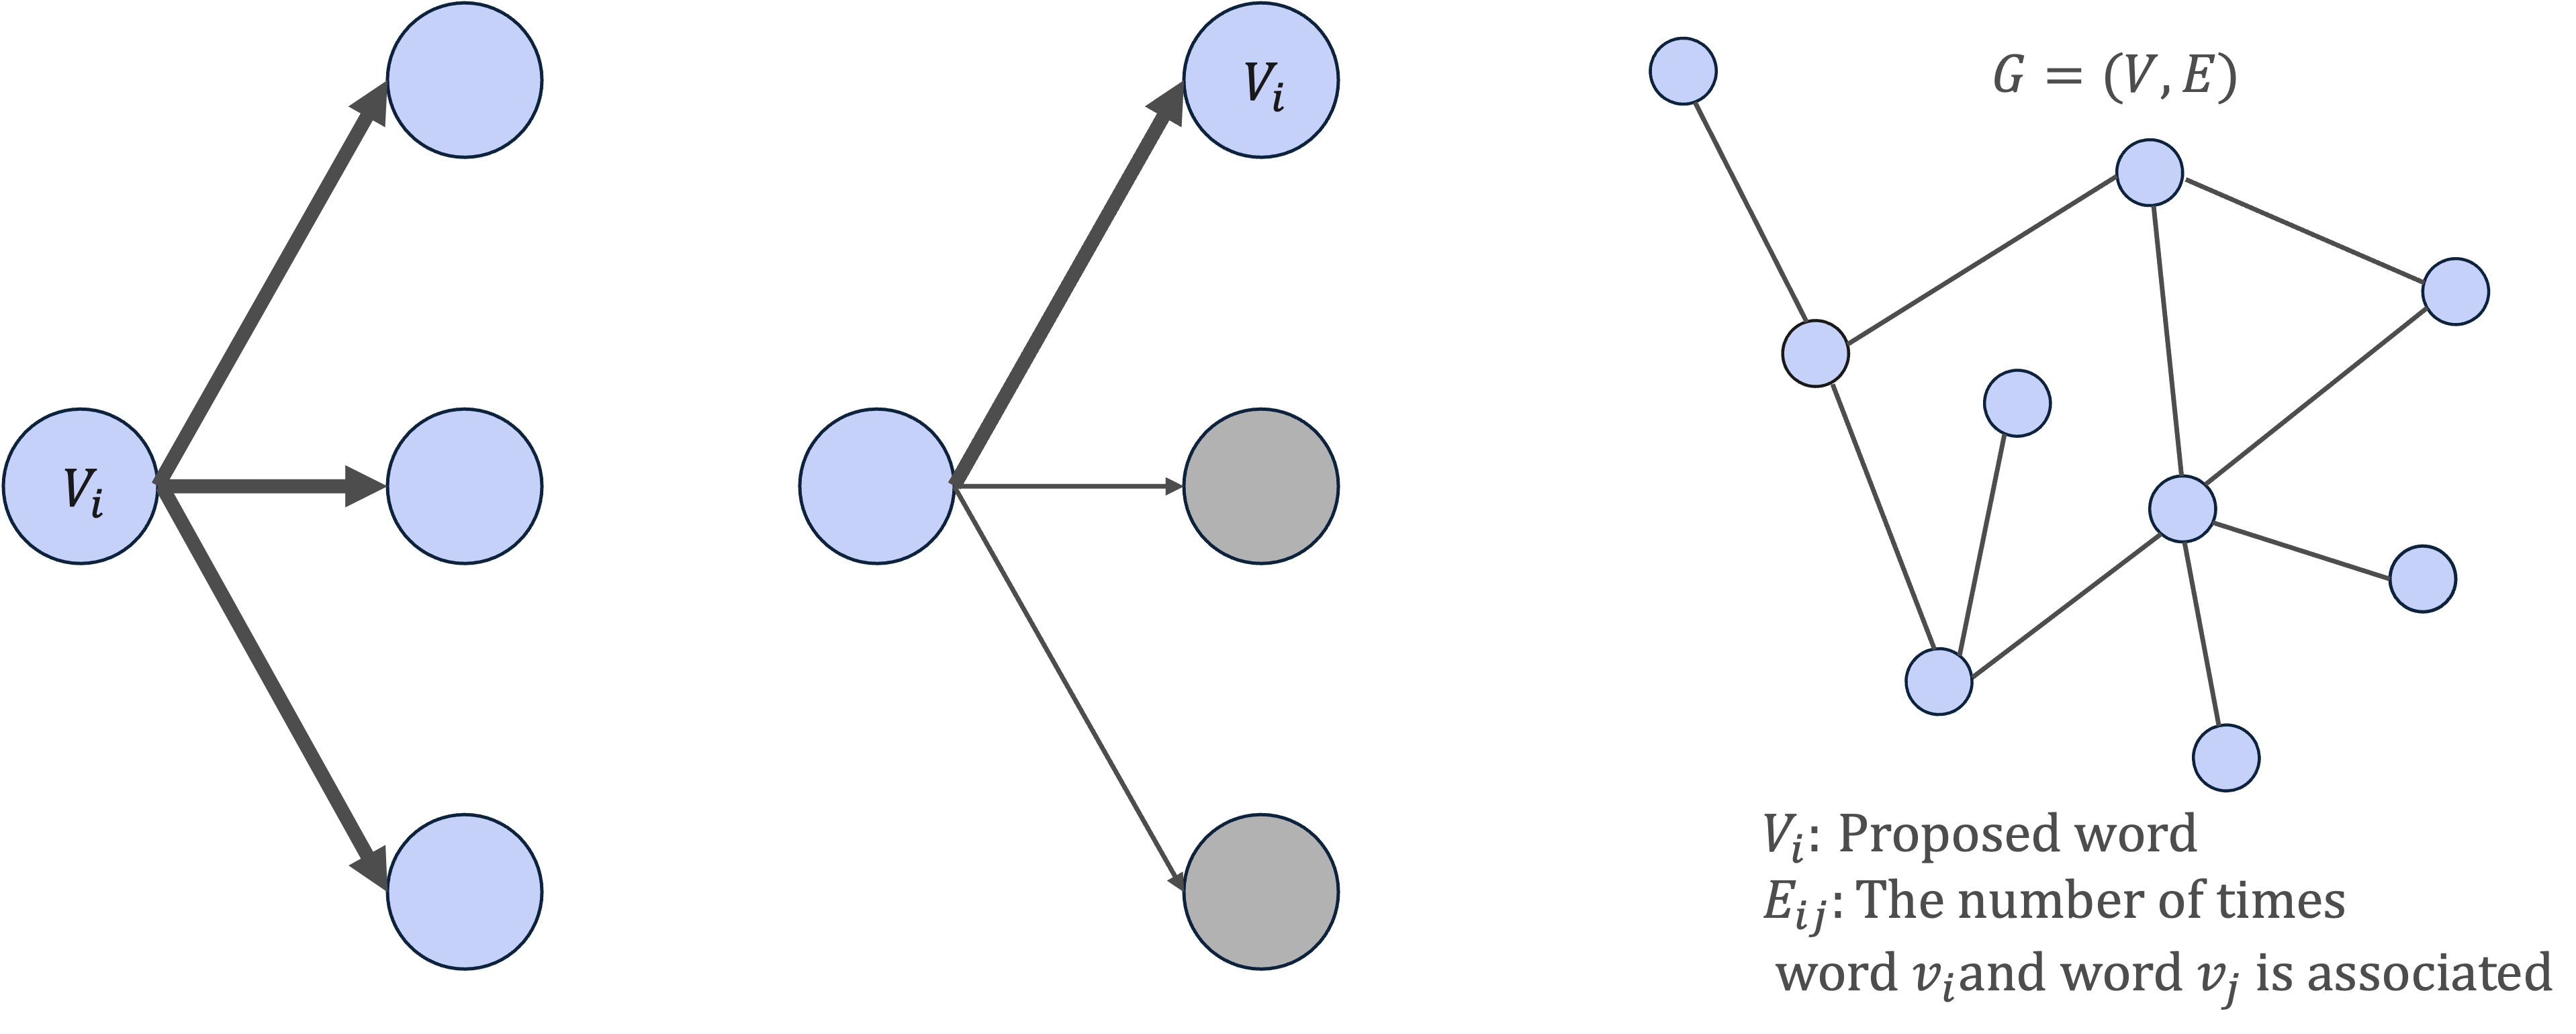
\includegraphics[width=0.7\linewidth]{Images/associate.png}
    %\caption{Consturct word-association network based on word association exercise}
    %\label{fig:association}
\end{figure}

\end{frame}
%------------------------------------------------

\begin{frame}
    \frametitle{Words-association Network}
    %\framesubtitle{Snowballing word association exercise and construction of network}
    \textbf{Conduct survey}
    \begin{itemize}        
        \item  Utilizing an online survey conducted in Japan, we engaged participants ranging from $20$ to $79$ years old and collected a total of $2,507$ responses.
        \begin{itemize}
            \item Participants were instructed to provide different words to the initial answer and to avoid responding in full sentences.	
        \end{itemize}
        \end{itemize}
        \pause
        \textbf{Data Processing}
        \begin{itemize}
        \item Remove invalid responses, such as “\textit{no idea}”, “\textit{don't know}”, or “\textit{none}”.
        \item Select words that are mentioned at least three times.
        \end{itemize}
        \pause
        \textbf{Network Construction}
        \begin{itemize}
        \item  Construct an \structure{undirected word association network} based on the data gathered from the responses. 
        \begin{itemize}
            \item Nodes represent the \textbf{words mentioned in the participants’ responses.}
            \item Edges imply the \textbf{associative connections between pairs of words.}
            \begin{itemize}
                \item These connections are weighted according to the frequency of their associations.
            \end{itemize}
        \end{itemize}
    \end{itemize}

\end{frame}

%------------------------------------------------

\begin{frame}
	\frametitle{Words-association Network}
	\framesubtitle{Using community detection to specify the components of well-being}
	\small % Reduce font size in this slide
	\begin{columns}[T] % [T] ensures correct vertical alignment
		\begin{column}{0.45\linewidth} % Left column
                   \centering
                   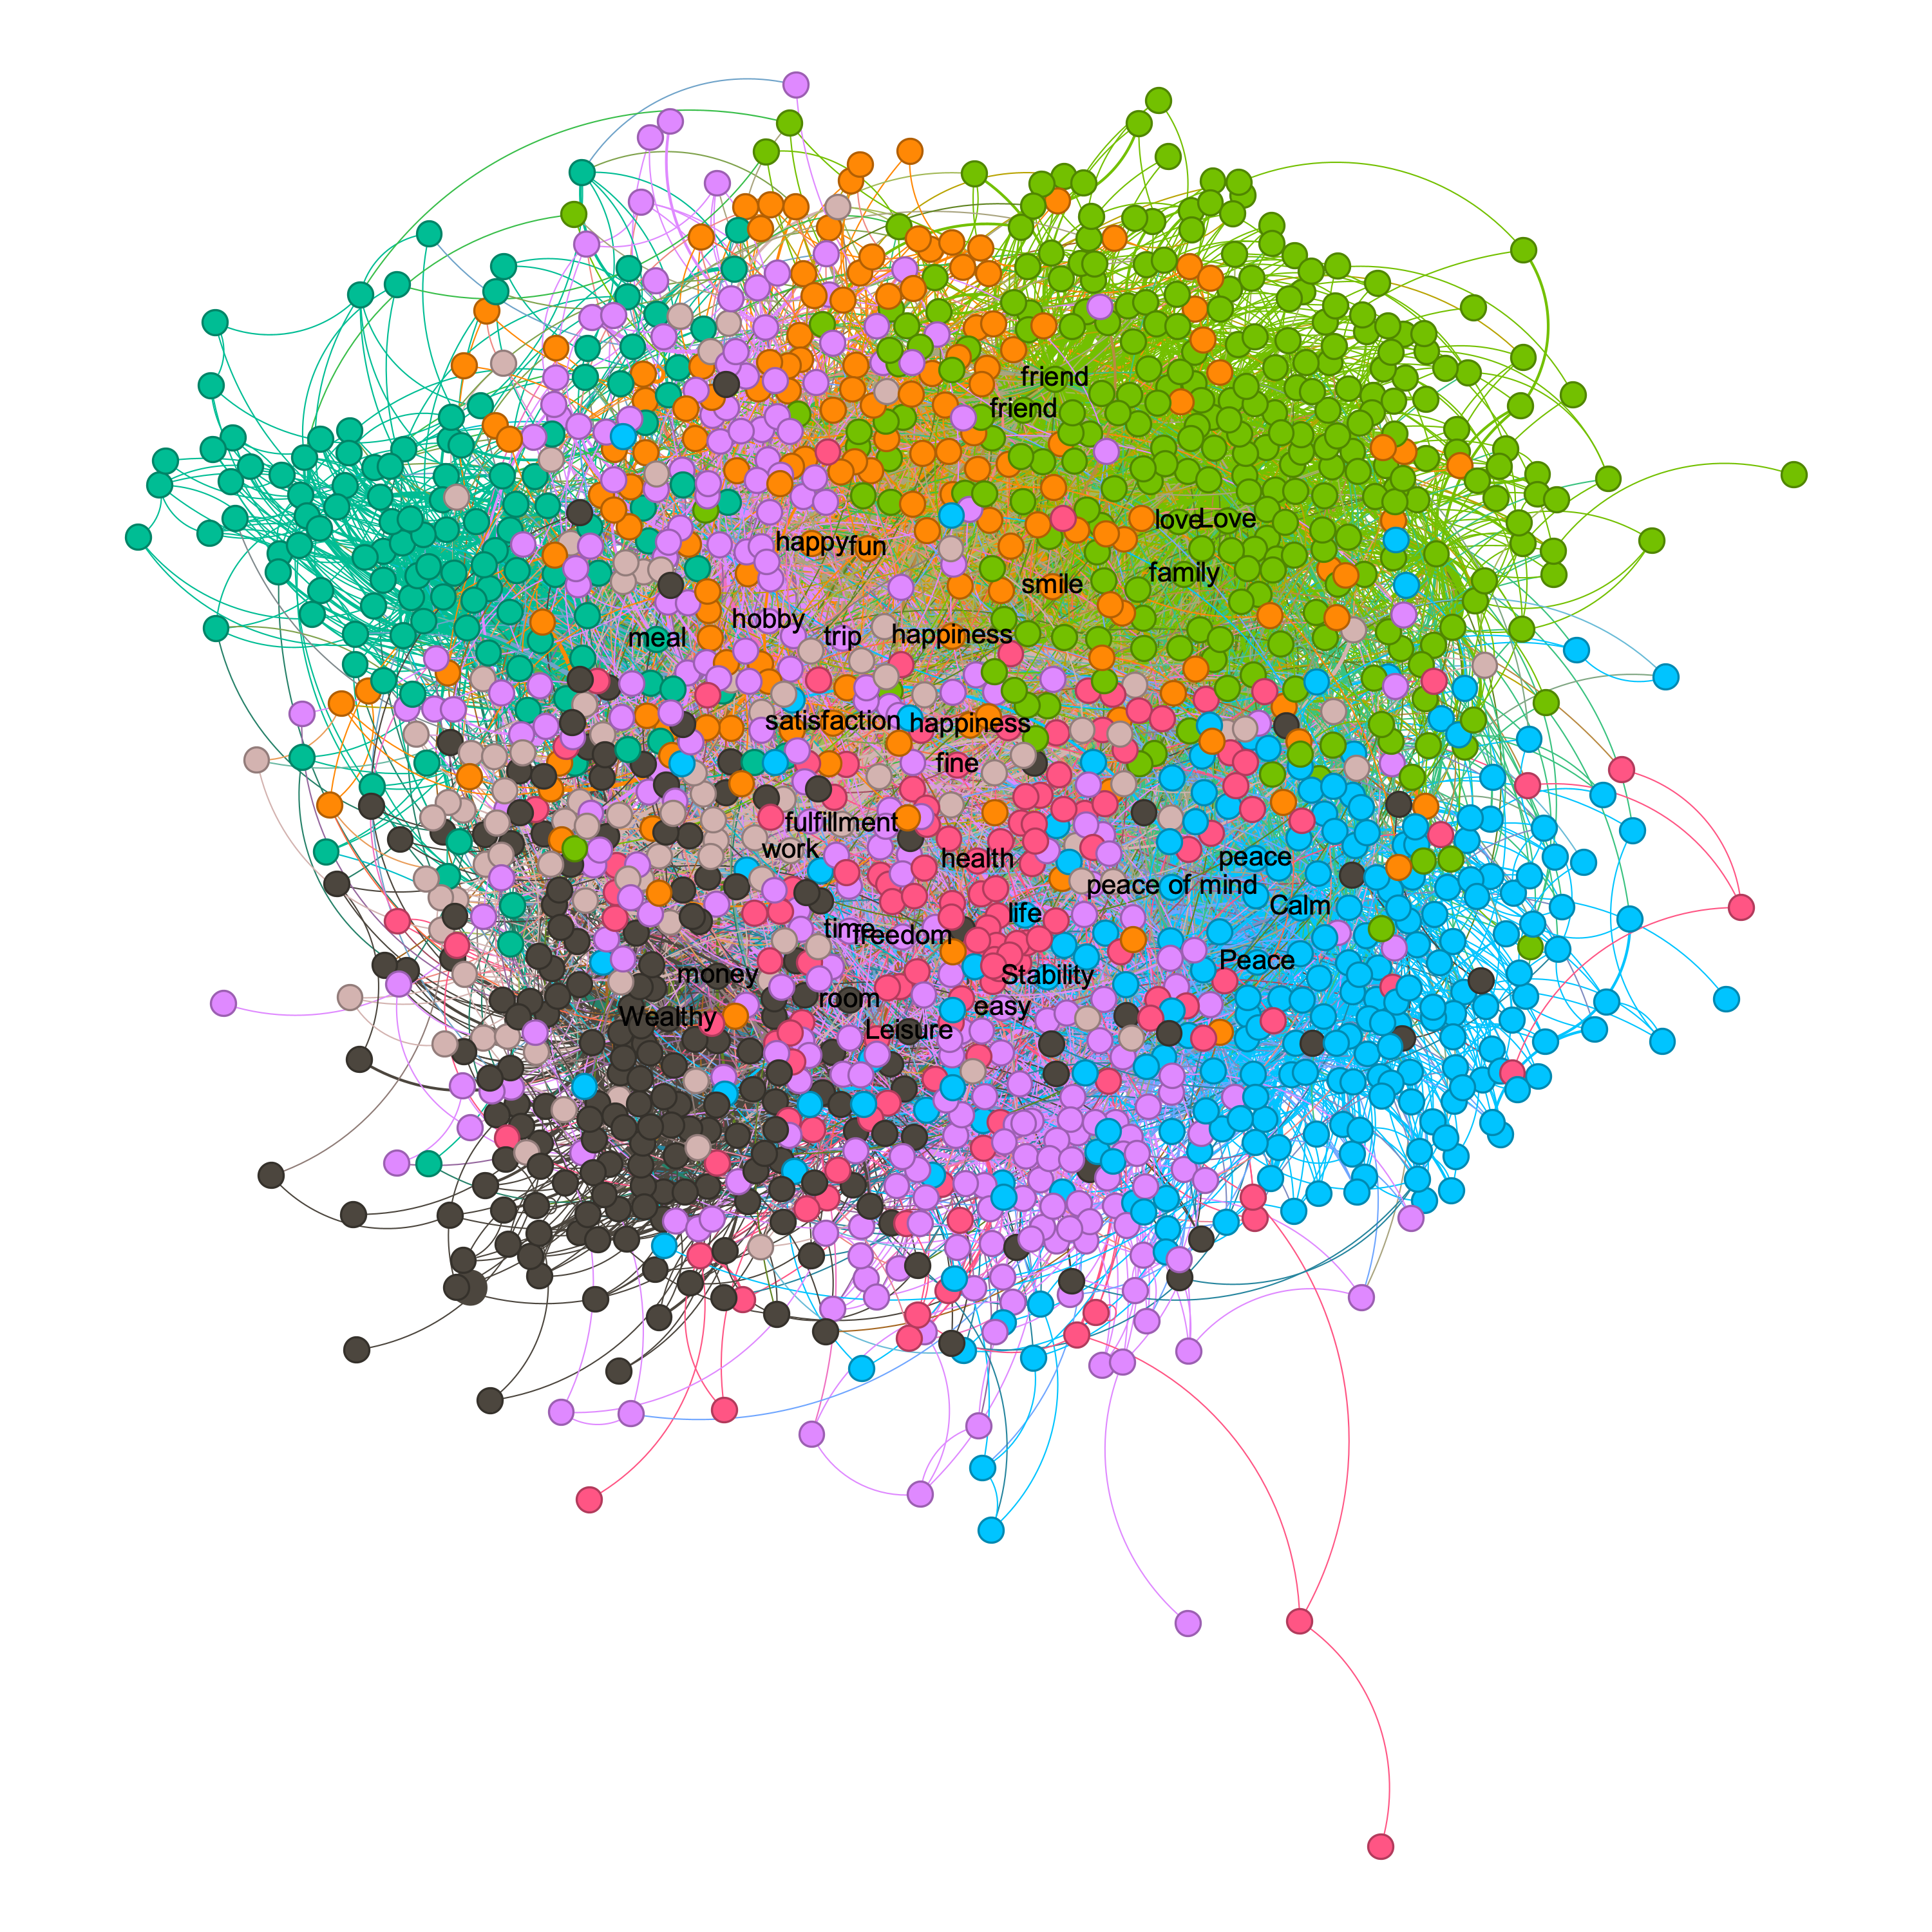
\includegraphics[width=0.5\linewidth]{Images/well_being_all_en.png}\\[1pt]

			\begin{itemize}
			    \item The Louvain algorithm is applied to identify communities within the word-association network.
                    \item Detected communities are interpreted as \structure{distinct components of well-being}.
                    \begin{itemize}
                        \item Words grouped within the same community are assumed to share close semantic and contextual relationships.
                    \end{itemize}
			\end{itemize}
		\end{column}
		\begin{column}{0.45\linewidth} % Center column
			\centering
                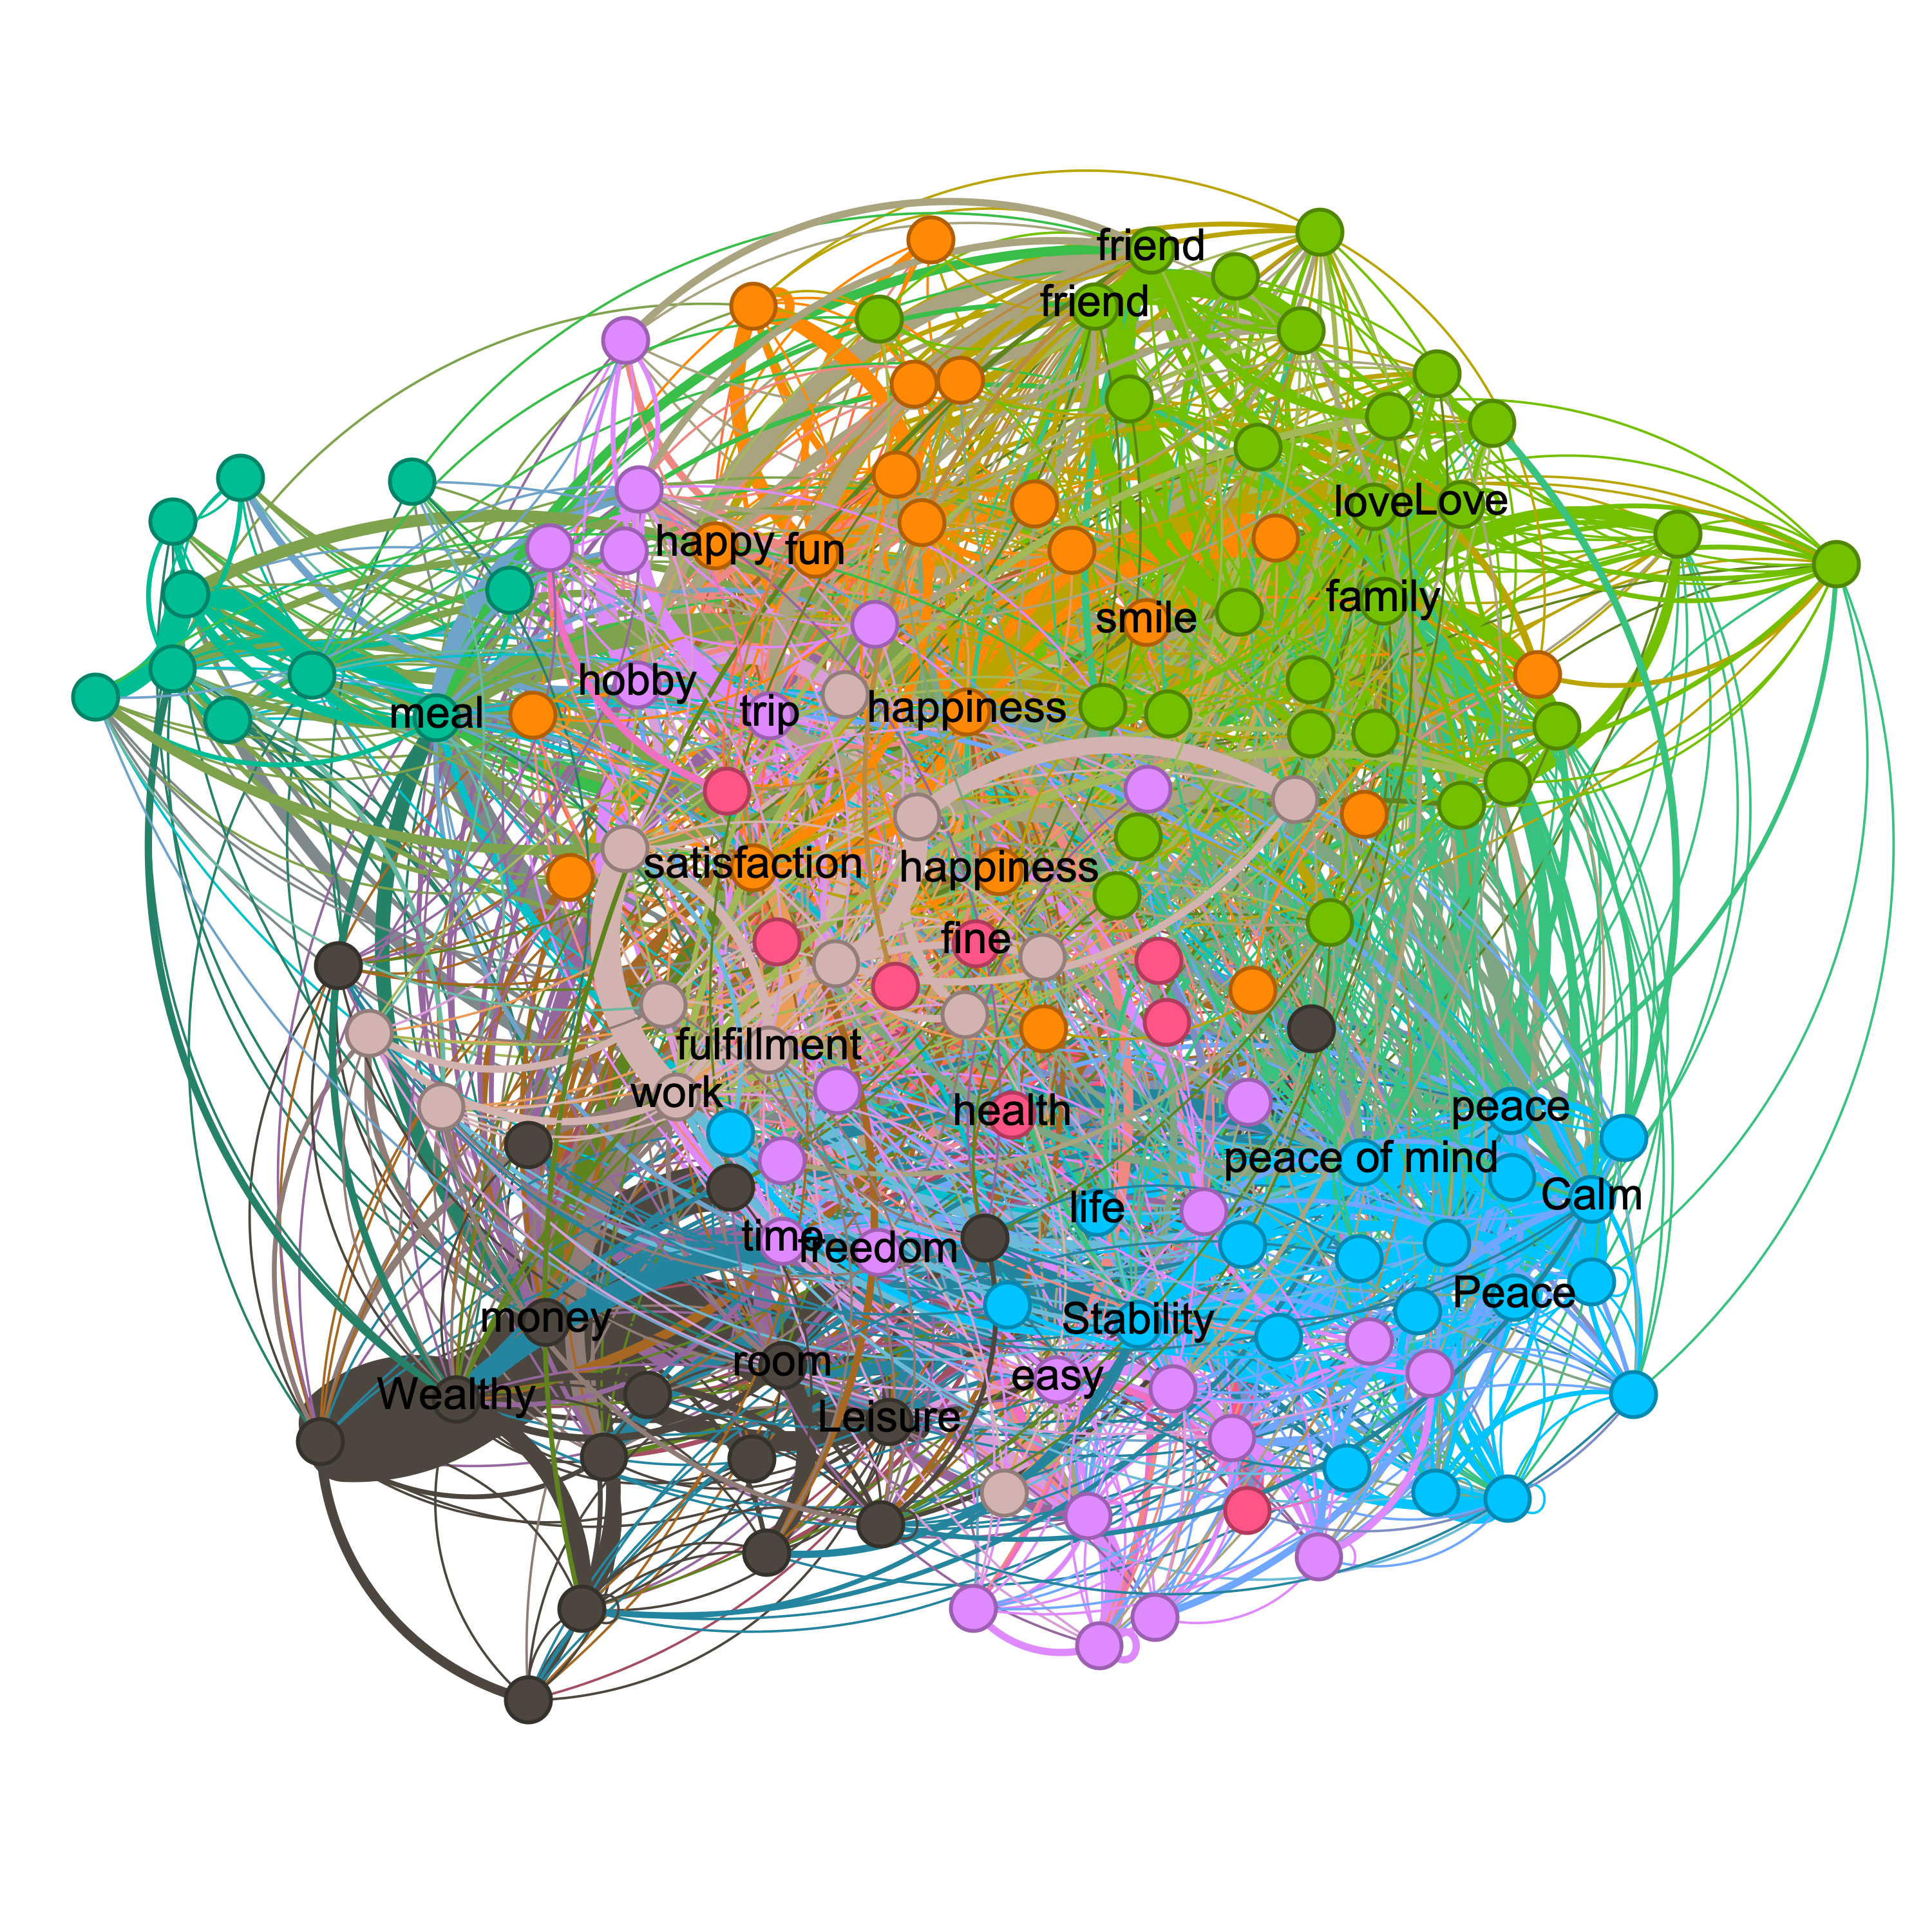
\includegraphics[width=0.5\linewidth]{Images/well_being_main_en.png}\\[1pt]
                \begin{itemize}
                    \item Identify the components of well-being based on key nodes in each community.
                    \item Eight key components of well-being, including 
                    \vspace{-0.75cm}
                    \begin{columns}
                        \begin{column}{0.5\linewidth}
                            \begin{itemize}
                                \item “\textit{Health}” 
                                \item “\textit{Achievement}”
                                \item “\textit{Pleasure}”
                                \item “\textit{Family/Friends}”
                            \end{itemize}
                        \end{column}
                        \begin{column}{0.5\linewidth}
                            \begin{itemize}
                                \item “\textit{Peacefulness}”
                                \item “\textit{Free/Leisure}”
                                \item “\textit{Wealth}”
                                \item “\textit{Food}”
                            \end{itemize}
                        \end{column}
                    \end{columns}
                \end{itemize}
		\end{column}
	\end{columns}
\end{frame}

\begin{frame}
    \frametitle{Words-association Network}
    \framesubtitle{Key words contained in the respective components of well-being network.}
    \vspace{1cm}
    \begin{table}
     \begin{center}
     \begin{tabular}{@{}ll@{}}
     \toprule
Community & Key Words (in English)\\
\midrule
Food & Meals, Fullness, Food, Eating, Delicious \\
Peacefulness & Peace, Stability, Serenity, Tranquility, Safety \\
Free/Leisure & Freedom, Hobby, Sleep, Travel, Time \\
Health & Health, Fine, Family's health, Comfort, Personal health \\
Wealth & Wealth, Affluence, Wealthy, Financial Freedom, Income \\
Pleasure & Joyful, Smiles, Happiness, Contentment, Laughter \\
Family/Friends & Family, Friends, Children, Love, Companions \\
Achievement & Work, Fulfillment, Hope, Dreams, Success \\
\bottomrule
\end{tabular}
\end{center}
\end{table}
    
\end{frame}

%------------------------------------------------
\section{Analysis}
%------------------------------------------------
\subsection{Constructs of well-being}

%------------------------------------------------

\begin{frame}
	\frametitle{Analysis on the constructs of well-being}
	\framesubtitle{Inter-community connectivity of word association network}
	
	\begin{columns}[T] % [T] ensures correct vertical alignment
		\begin{column}{0.48\linewidth} % Left column
			\textbf{Inter-community connections}
                $$
                \frac{total\ edge\ weights\ between\ two\ communities\ }{total\ edge\
weights\ within\ each\ community}
                $$
                \vspace{-0.75cm}
                \begin{itemize}
                    \item Inter-community connectivity informed the relationship among components.
                    \item A higher value indicates a closer relationship.
                    \pause
                    \begin{itemize}
                        \item “\textit{Pleasure}” shows relatively high connectivity with components “\textit{Free/Leisure}” and “\textit{Family and Friends}”
                        \item “\textit{Pleasure}” ($0.301$) have the highest average inter-community connectivity among components.
                    \end{itemize}
                \end{itemize}
		\end{column}
		\begin{column}{0.48\linewidth} % Right column
			%\vspace{-3.5\baselineskip} % Pull image up
			
			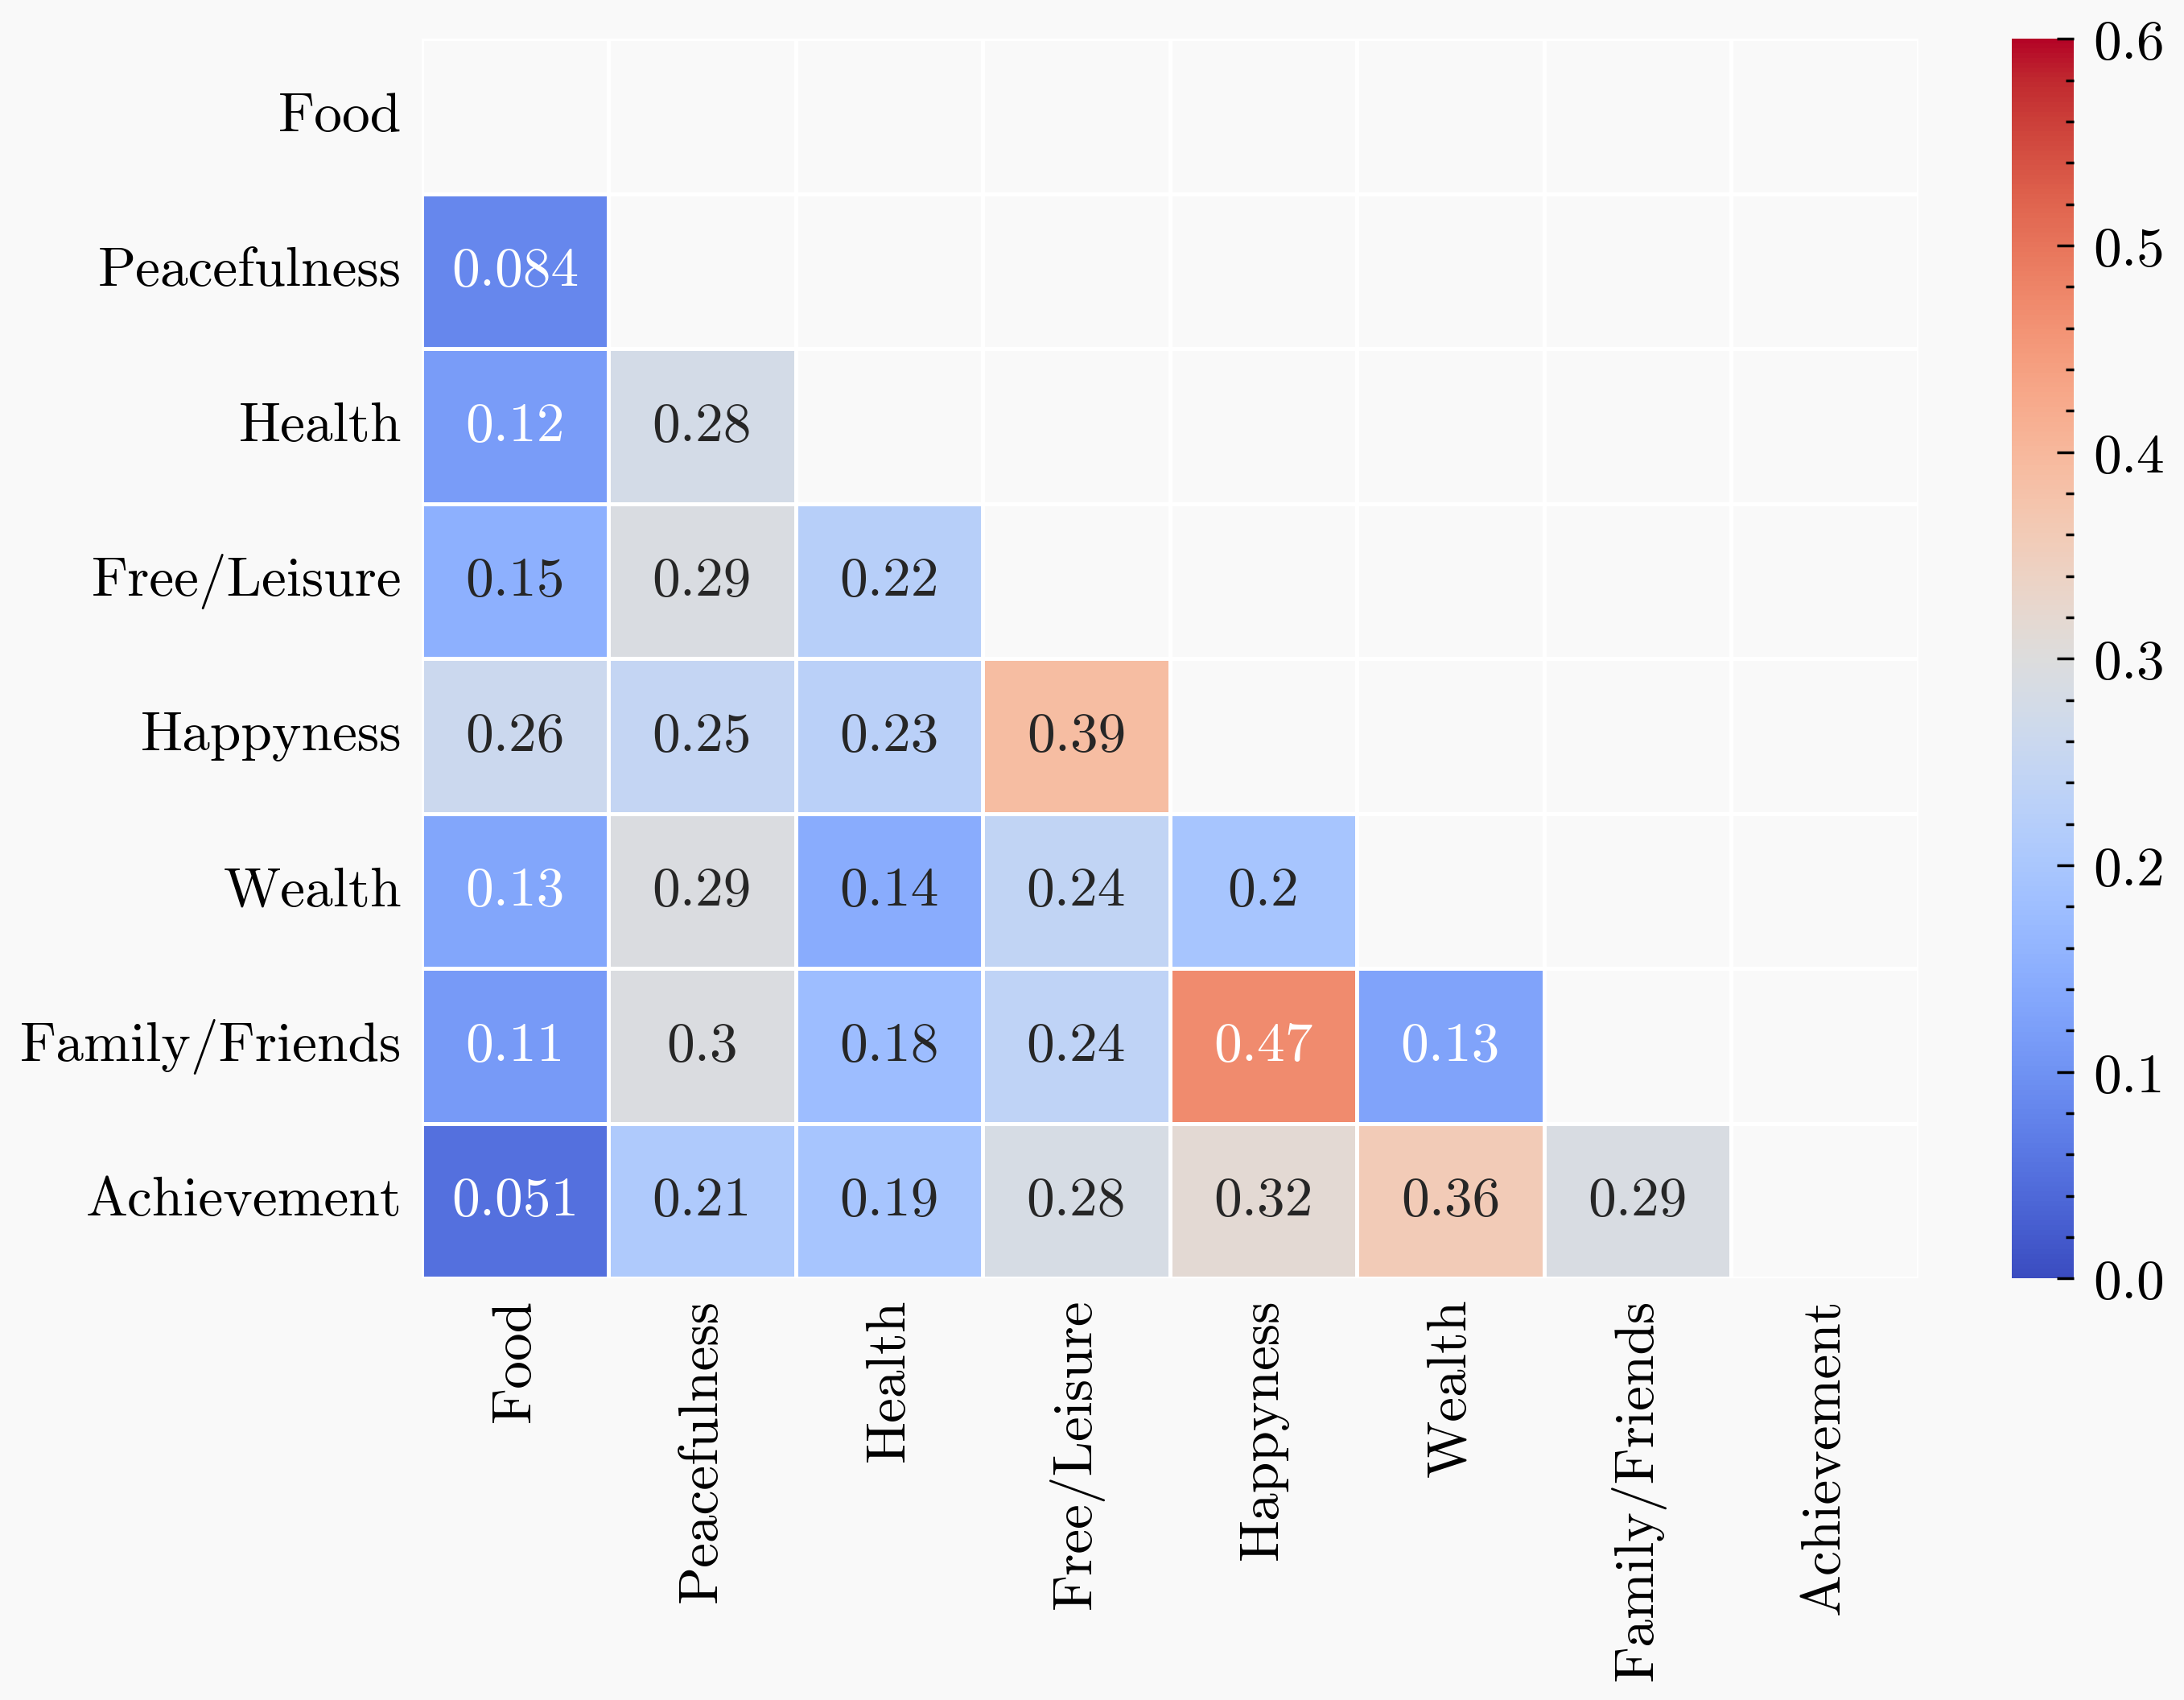
\includegraphics[width=\linewidth]{Images/well_being_corr.png} % Trimming is used to crop your image and the order of dimensions is: left, bottom, right, top. It's recommended to crop outside of LaTeX though, to ensure the aspect ratio remains the same.
			%{\tiny\textcolor{ICLBlue}{(Above) Photography Credit or Caption}}
		\end{column}
	\end{columns}
\end{frame}

%------------------------------------------------

%------------------------------------------------
\subsection{Demographic differences in the structure of well-being}

%------------------------------------------------
\begin{frame}
    \frametitle{Analysis on demographic differences}
    \framesubtitle{Demographic differences in each component of well-being}
    \begin{itemize}
        \item Most proposed words can be classified into specific components of well-being.
        \item Quantify the number of distinct well-being components referenced by each participant.
    \end{itemize}
    \pause
    
    $$
        W_i = \beta_{0}+\beta_{1}X_{j}+\epsilon
    $$
    \vspace{-1.5\baselineskip}
    \begin{itemize}
        \item  $W_i$ denotes the number of proposed words related to the component (community) of well-being $i$
        \item $X_{j}$ refers to the demographic characteristics of participant $j$
        \begin{itemize}
            \item Gender: $1$ indicates male and $0$ indicates female.
            \item Age: Categorized into ranges from the 20s to the 70s, with the 20s serving as the reference category in the regression model. 
            \item Education attainment: Categorical variable converted into the numerical format, representing levels from \textit{junior high school} ($1$) to \textit{graduate school} ($6$)
            \item Income: Categorical variable converted into the numerical format, indicating income levels from \textit{no income} ($1$) to \textit{over 12 million yen per year} ($15$).
        \end{itemize}
    \end{itemize}
    
\end{frame}
%------------------------------------------------


\begin{frame}
	\frametitle{Analysis on demographic differences}
	\framesubtitle{Difference in the perception of well-being between males and females}
	
	\begin{columns}[T] % [T] ensures correct vertical alignment
		\begin{column}{0.6\linewidth} % Left column
			%\textbf{Inter-community connections}
                \begin{itemize}
                    \item Compared to males, females place greater value on “\textit{Family and Friends}” and “\textit{Pleasure}” as key components of well-being, highlighting the significant role that \structure{social networks and emotional states play in females' lives}.
                    \begin{itemize}
                        \item Previous studies have suggested that females are typically more sensitive to psychological and affect issues and are more inclined to seek emotional support from their close persons \citep{fuhrerGenderSocialRelations1999,bedrov_thriving_2022}.
                    \end{itemize}
                    \item \structure{Males are more likely to consider “\textit{Wealth}”} an important component of well-being
                    \begin{itemize}
                        \item Societal expectations and self-identity that demand economic resources from males \citep{zyphur_income_2015,crowley_mens_1998,lee_demographic_2022}
                    \end{itemize}
                \end{itemize}
		\end{column}
		\begin{column}{0.35\linewidth} % Right column
			\vspace{-1\baselineskip} % Pull image up
			\hspace{-1\baselineskip}
			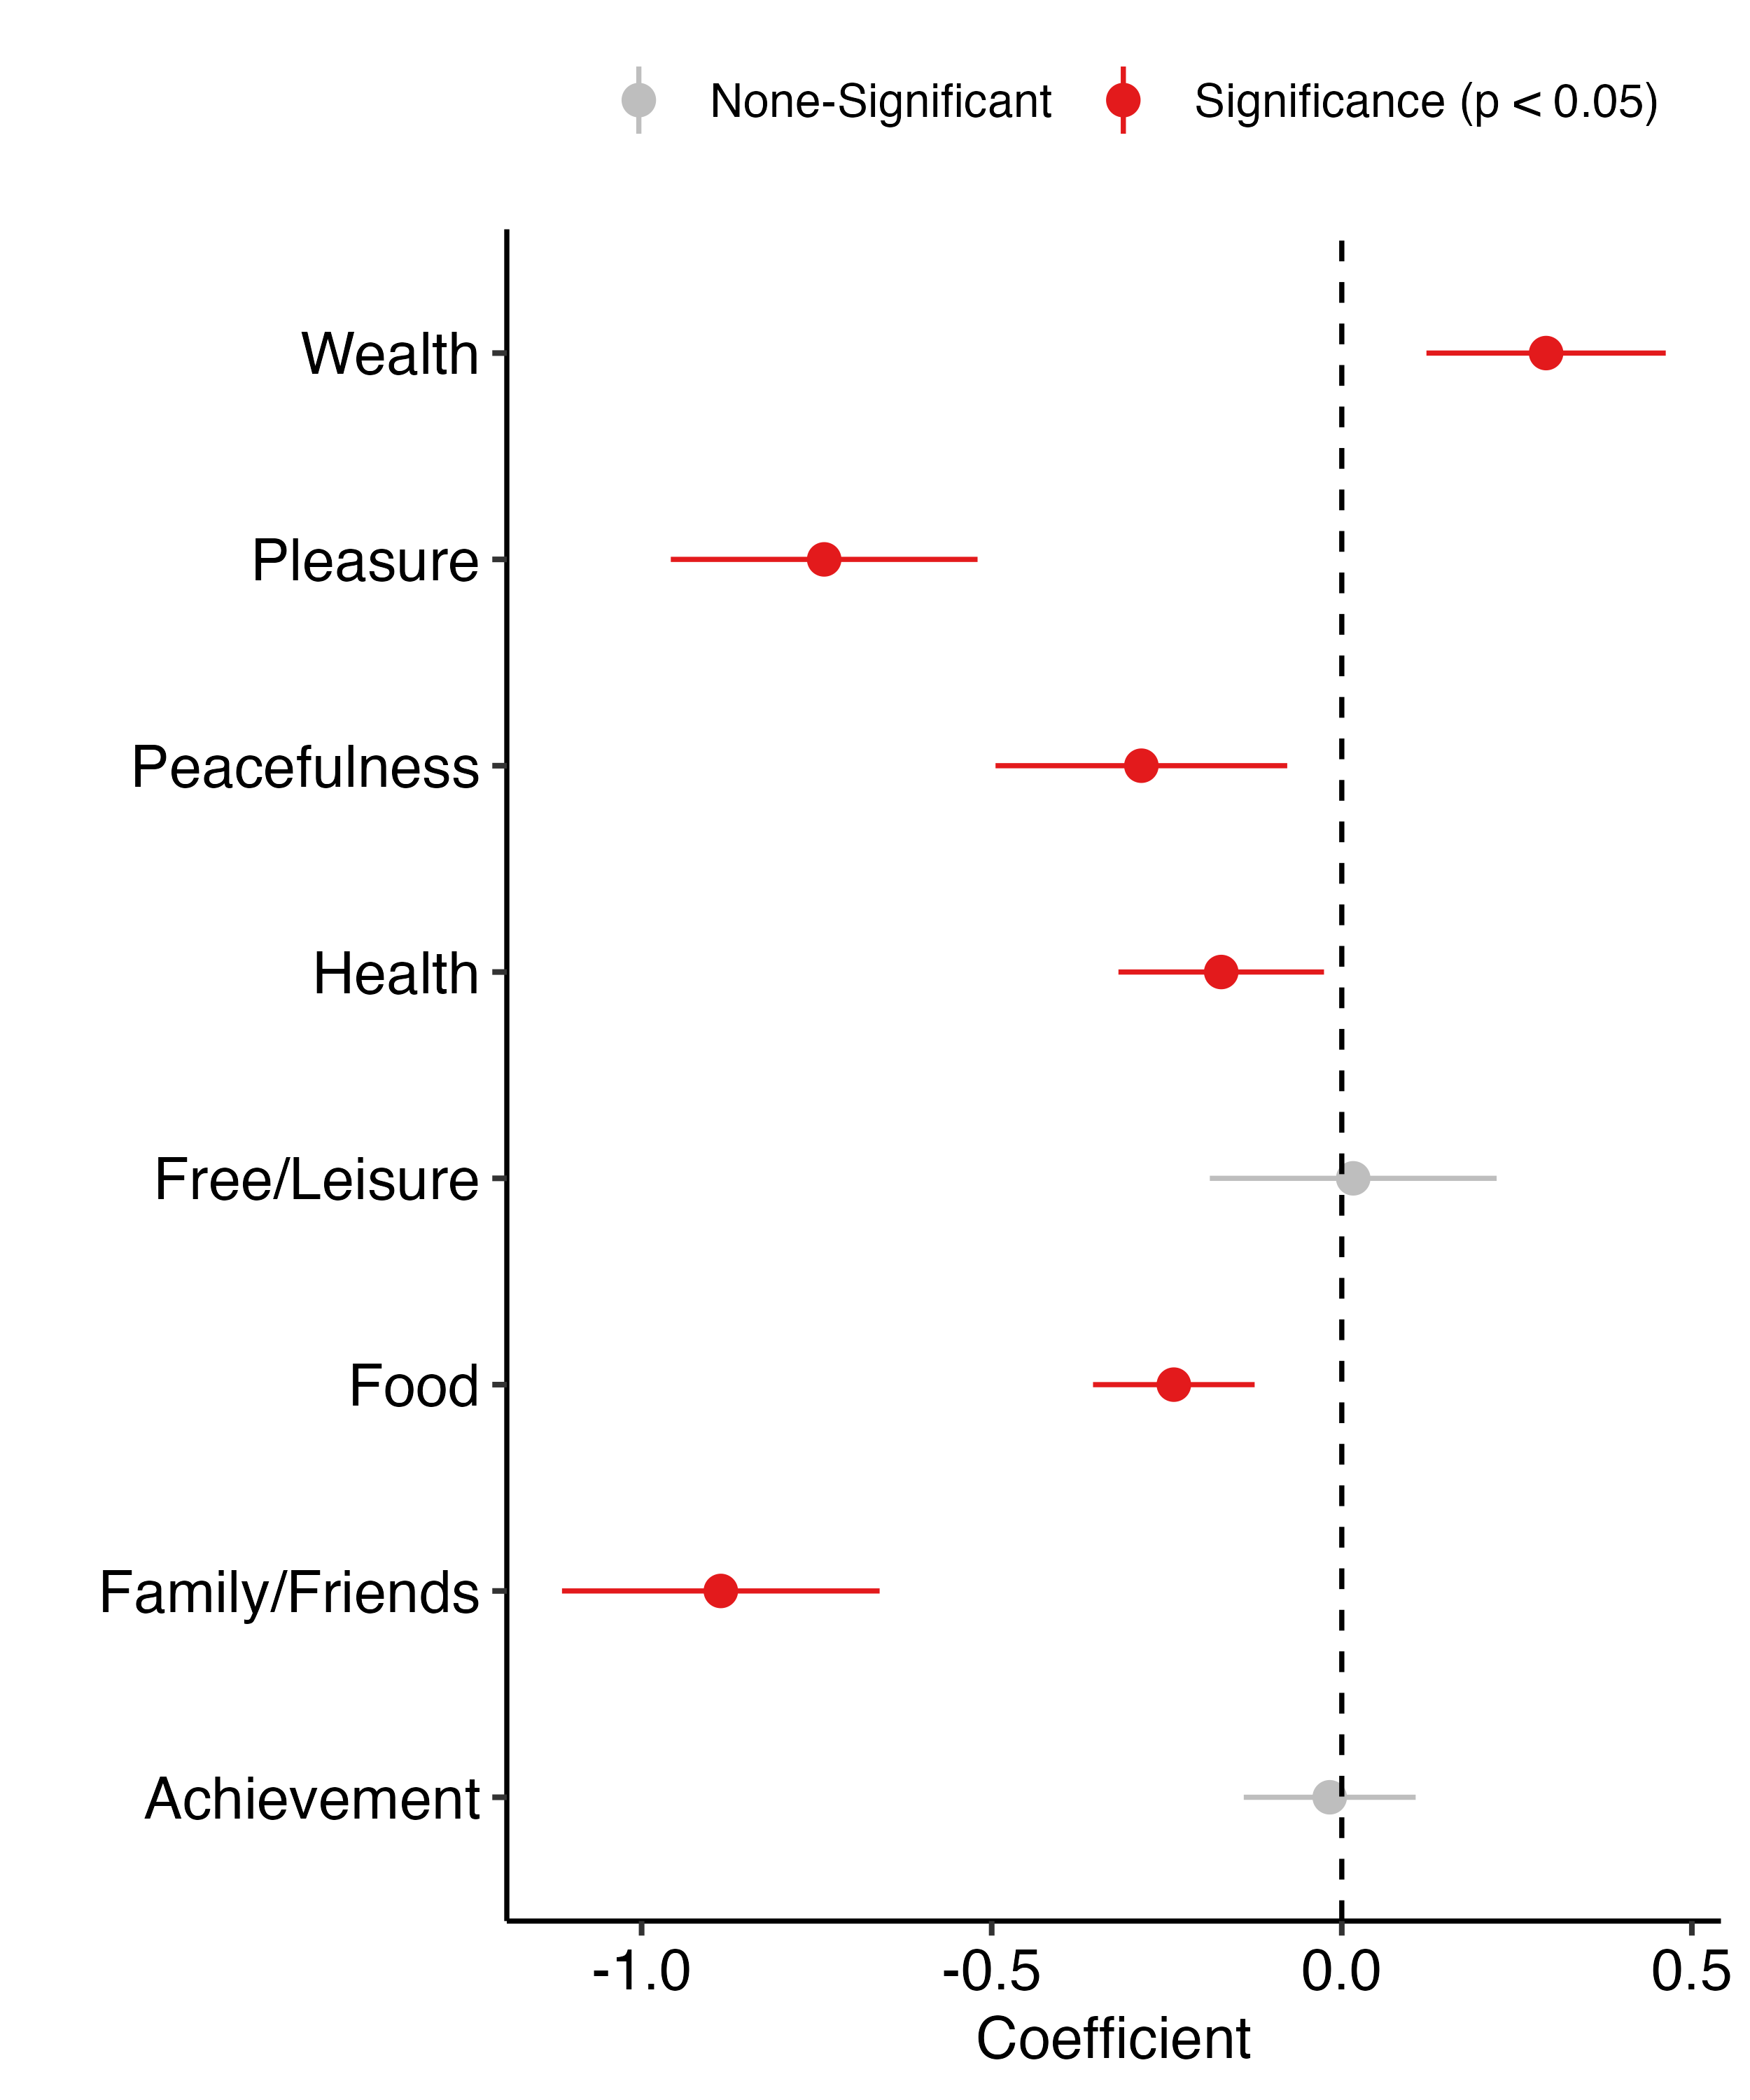
\includegraphics[width=\linewidth]{Images/well_being_community_gender.png} % Trimming is used to crop your image and the order of dimensions is: left, bottom, right, top. It's recommended to crop outside of LaTeX though, to ensure the aspect ratio remains the same.
			%{\tiny\textcolor{ICLBlue}{(Above) Photography Credit or Caption}}
		\end{column}
	\end{columns}
\end{frame}

%------------------------------------------------
\begin{frame}
	\frametitle{Analysis on demographic differences}
	\framesubtitle{Difference in the perception of well-being among different age groups}
	\begin{columns}[T] % [T] ensures correct vertical alignment
		\begin{column}{0.48\linewidth} % Right column
			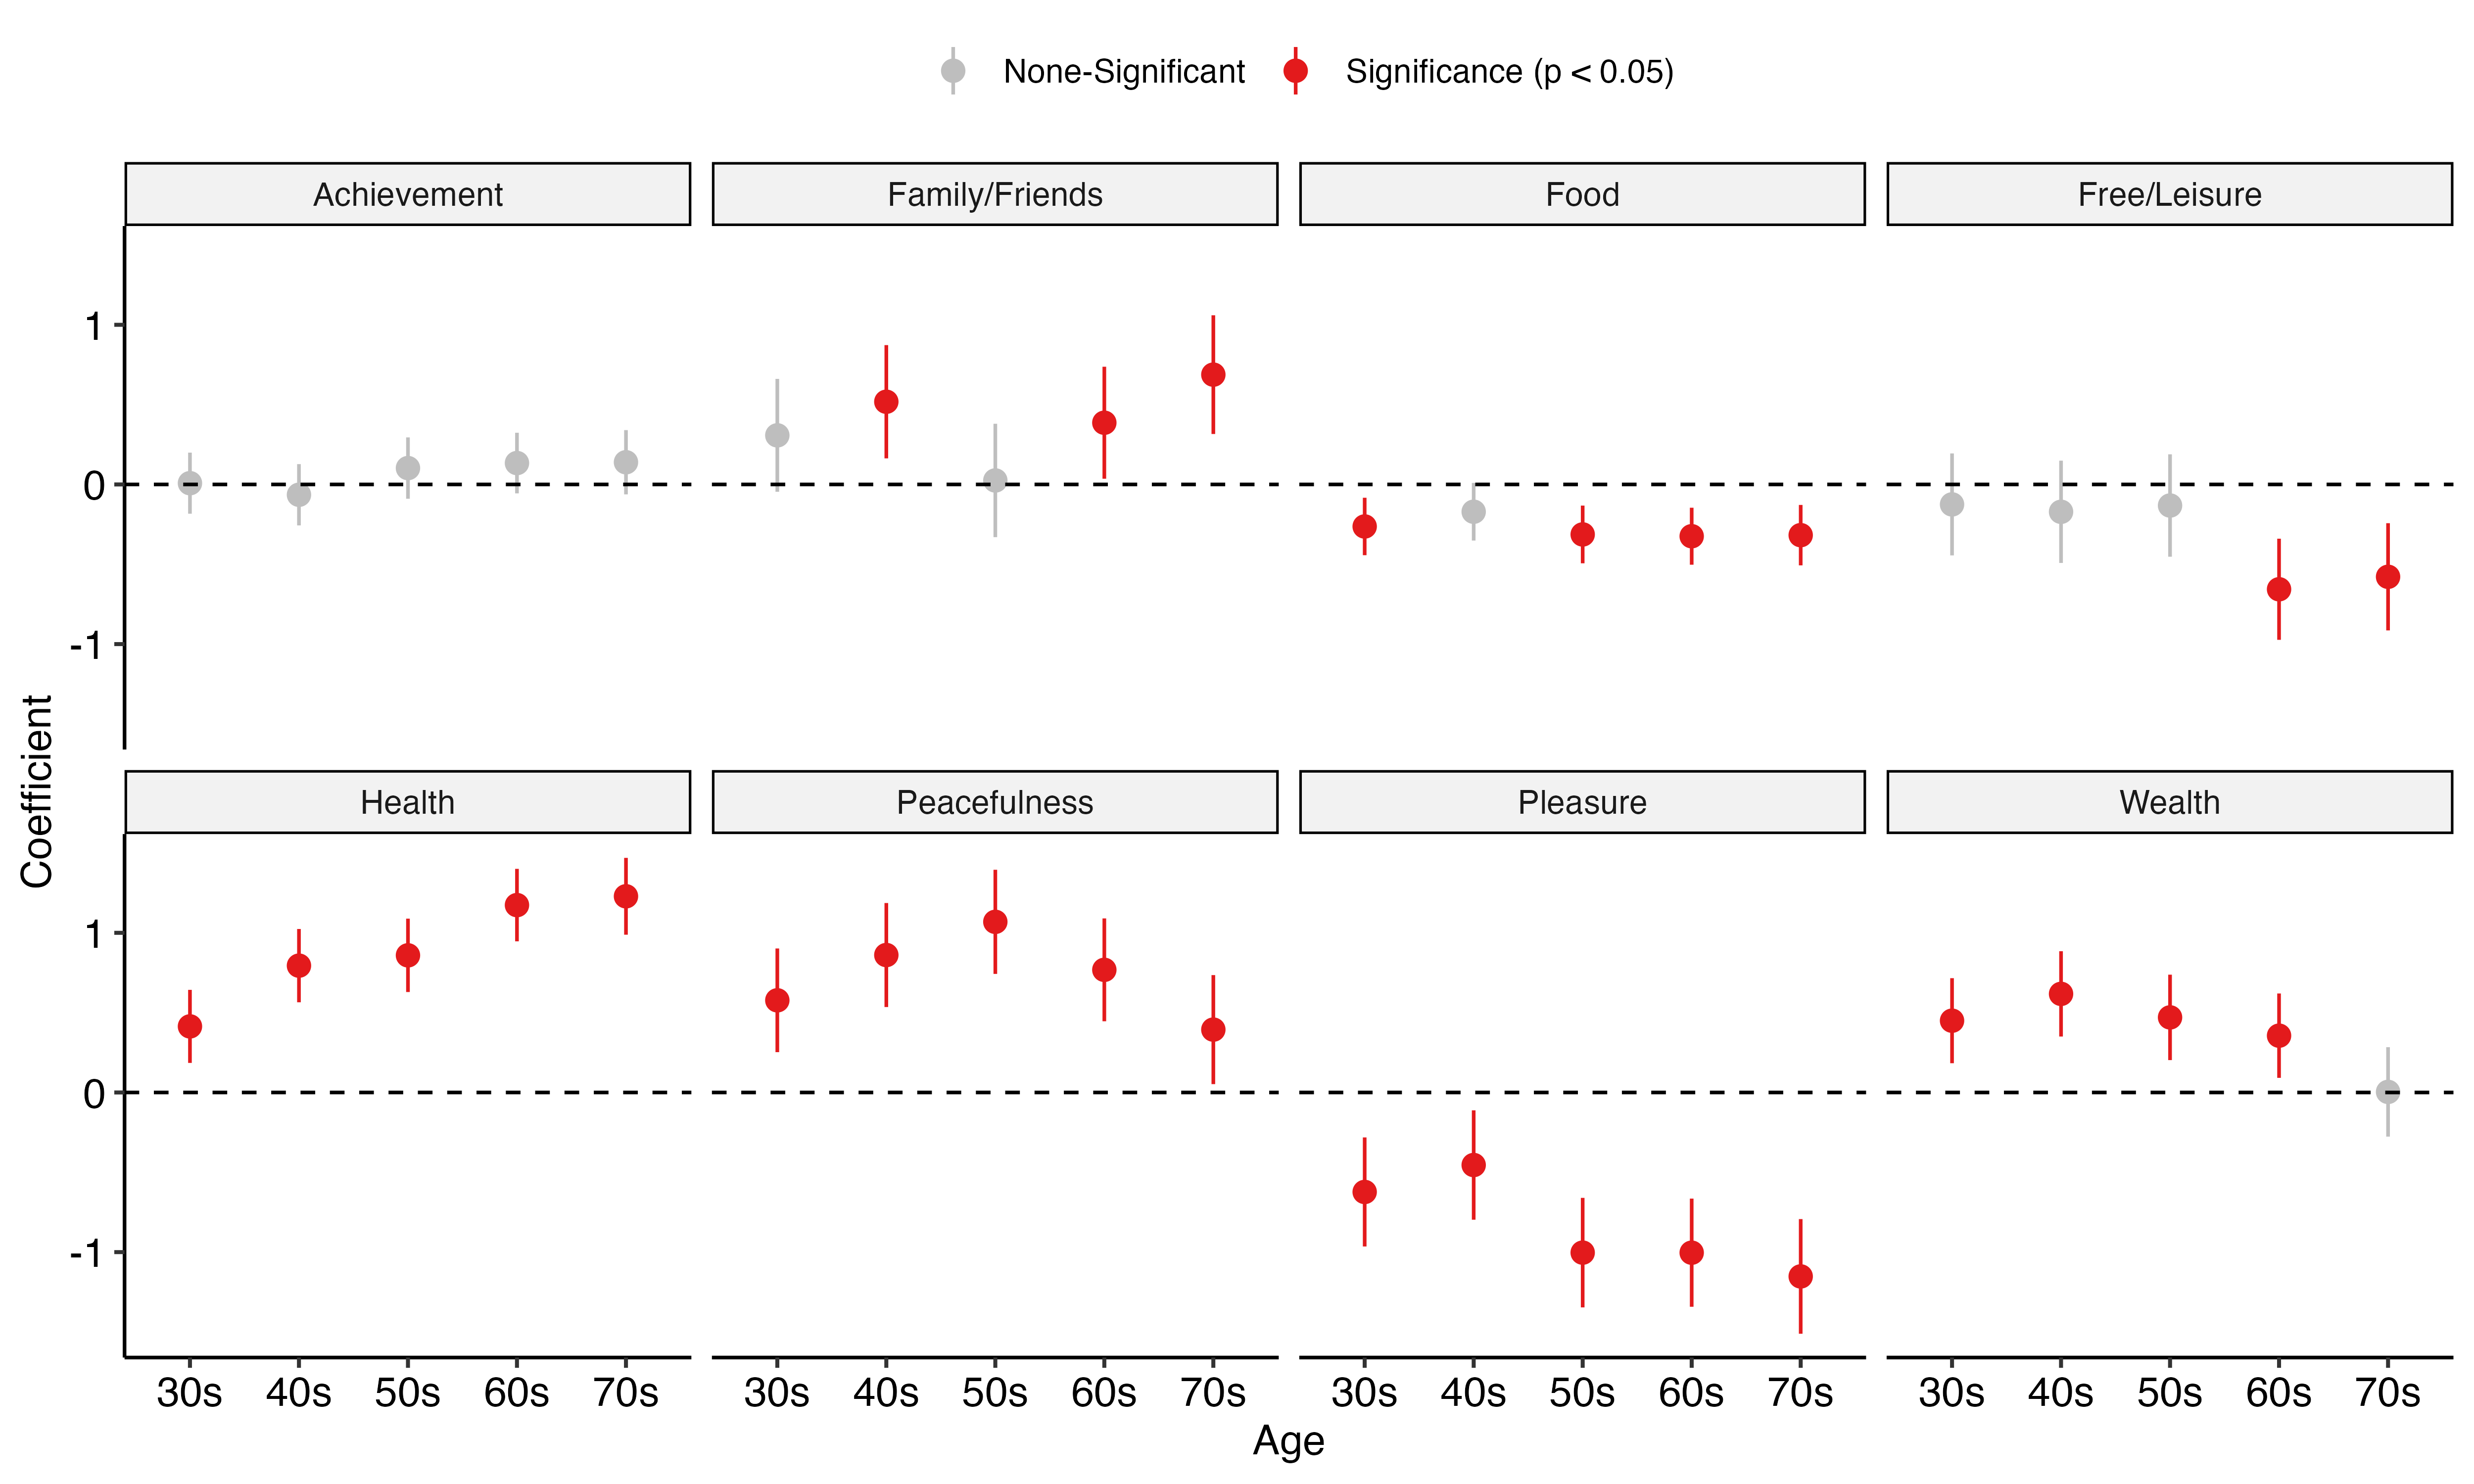
\includegraphics[width=\linewidth]{Images/well_being_community_age_p.png} 
            \vspace{-1.5\baselineskip} 
            \begin{itemize}
                \item Many factors that inhibit well-being exist in the life experiences of the middle-aged period.
                \begin{itemize}
                    \item U-shaped trajectory throughout life \citep{steptoe_psychological_2015}
                \end{itemize}
            \end{itemize}
		\end{column}
            \pause
            \begin{column}{0.48\linewidth} % Left column
			%\textbf{Inter-community connections}
                \begin{itemize}
                    \item  Middle-aged individuals, those in their 30s to 50s, are more inclined to \structure{associate well-being with “\textit{Wealth}” compared to people in their 20s and 70s.}
                    \begin{itemize}
                        \item Sacrifice current well-being during middle age \citep{steptoe_psychological_2015}
                    \end{itemize}
                    \pause
                    \item With age increased, people increasingly emphasize the importance of \structure{"\textit{Health}".}
                        \begin{itemize}
                            \item The increasing prominence of health issues may lead to decreased well-being among middle-aged individuals.
                        \end{itemize}
                    \item Middle-aged individuals still have a significant need for \structure{"\textit{Freedom/Leisure}".}
                    \begin{itemize}
                        \item Work responsibilities and economic pressures often prevent these needs from being fully realized.
                    \end{itemize}
                \end{itemize}
		\end{column}
	\end{columns}
\end{frame}
%------------------------------------------------

%------------------------------------------------

\begin{frame}
	\frametitle{Analysis on demographic differences}
	\framesubtitle{How perception of well-being related to educational attainment}
	
	\begin{columns}[T] % [T] ensures correct vertical alignment
		\begin{column}{0.6\linewidth} % Left column
			%\textbf{Inter-community connections}
                \begin{itemize}
                    \item Individuals with higher educational attainment usually place a greater emphasis on \structure{"\textit{Health}"} as a crucial component of well-being
                    \begin{itemize}
                        \item  The emphasis on health issues could result in varying health outcomes among individuals with different levels of educational attainment \citep{zajacova_relationship_2018,hui_influence_2022,raghupathi_influence_2020}
                    \end{itemize}
                    \item Individuals with higher educational attainment tend to associate \structure{"\textit{Freedom/Leisure}"} and \structure{"\textit{Peacefulness}"} with well-being.
                    \begin{itemize}
                        \item Education enables access to resources that enhance well-being \citep{link_social_1995}
                    \end{itemize}
                    \pause
                    \item Individuals with higher educational attainment tend to associate \structure{“\textit{Achievement}”} with well-being
                    \begin{itemize}
                        \item Education can enhance eudaimonic well-being \citep{miquelon_goal_2006}
                    \end{itemize}
                \end{itemize}
		\end{column}
		\begin{column}{0.35\linewidth} % Right column
			\vspace{-1\baselineskip} % Pull image up
			
			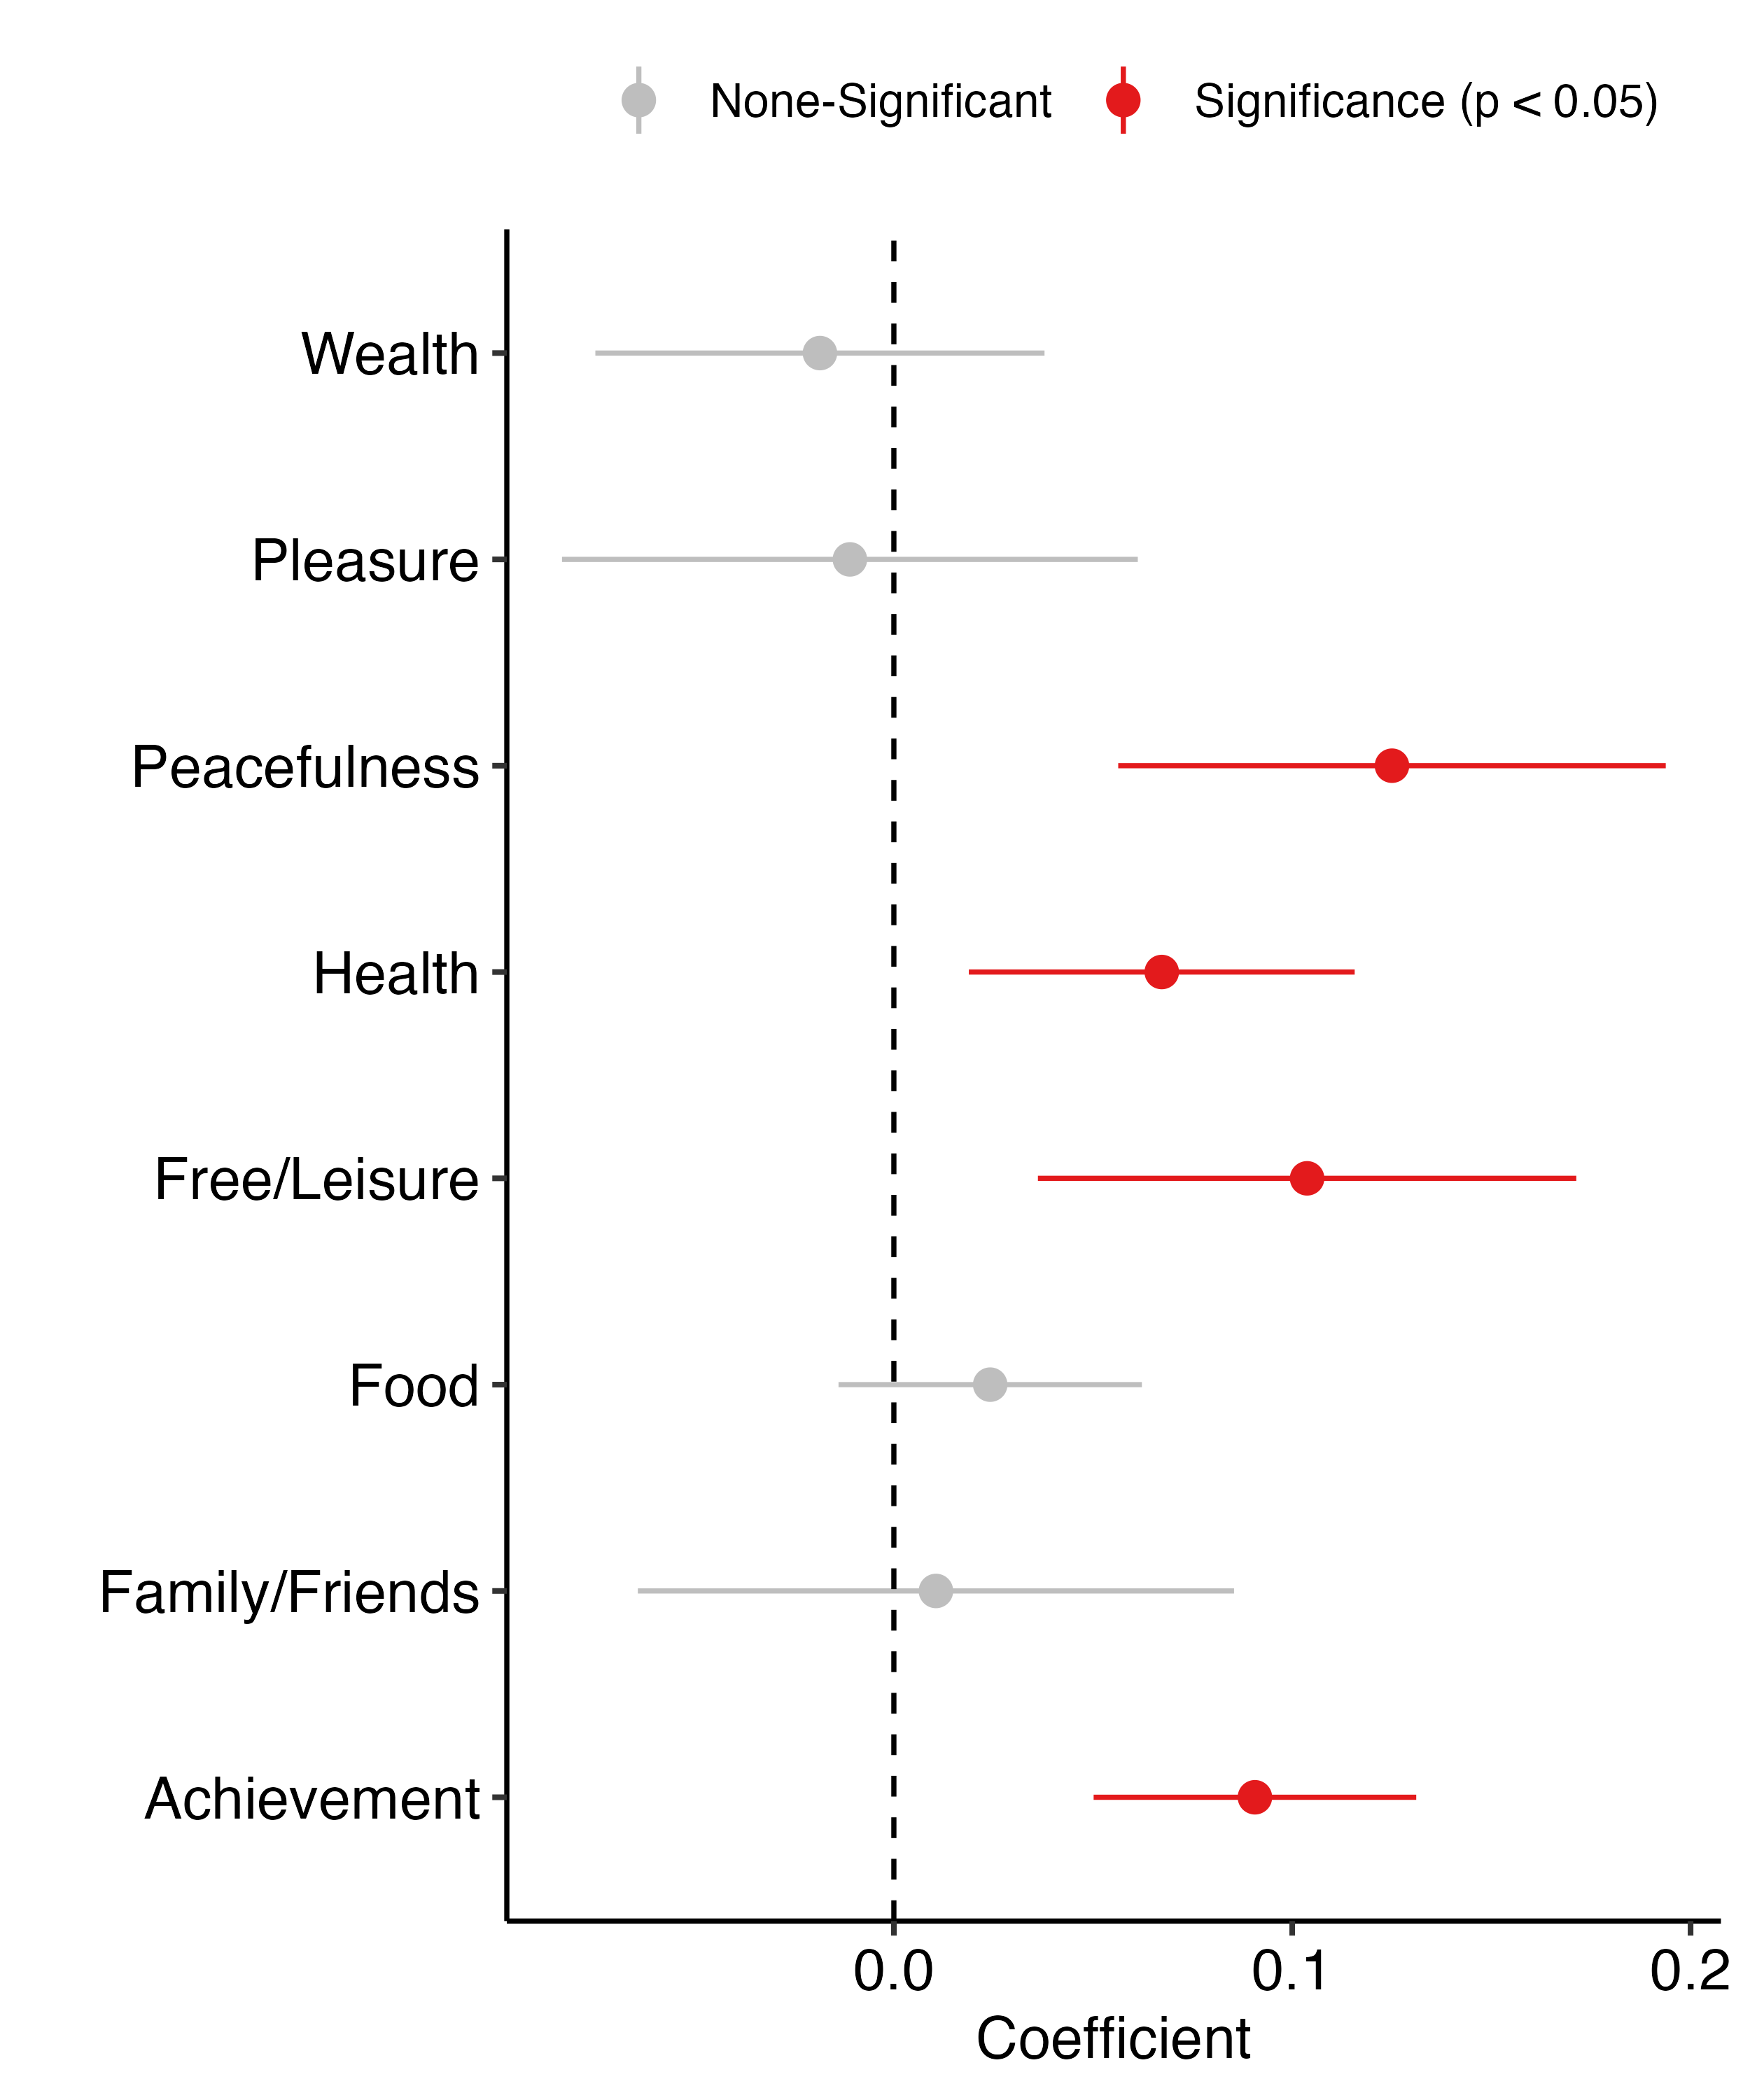
\includegraphics[width=\linewidth]{Images/well_being_community_edu.png} % Trimming is used to crop your image and the order of dimensions is: left, bottom, right, top. It's recommended to crop outside of LaTeX though, to ensure the aspect ratio remains the same.
			%{\tiny\textcolor{ICLBlue}{(Above) Photography Credit or Caption}}
		\end{column}
	\end{columns}
\end{frame}

%------------------------------------------------
%------------------------------------------------

\begin{frame}
	\frametitle{Analysis on demographic differences}
	\framesubtitle{How perception of well-being related to Income}
	
	\begin{columns}[T] % [T] ensures correct vertical alignment
		\begin{column}{0.6\linewidth} % Left column
			%\textbf{Inter-community connections}
                \vspace{2.5\baselineskip}
                \begin{itemize}
                    \item Individuals with a higher income are more likely to emphasize \structure{“\textit{Achievement}”} as an important component of well-being.
                    \begin{itemize}
                        \item  Similar to educational attainment
                        \item  Income can enhance \textbf{eudaimonic well-being.}
                        \item  The recognition and respect they receive from others for their achievements can significantly boost their self-esteem and overall sense of well-being.
                    \end{itemize}         
                \end{itemize}
		\end{column}
		\begin{column}{0.35\linewidth} % Right column
			\vspace{-1\baselineskip} % Pull image up
			
			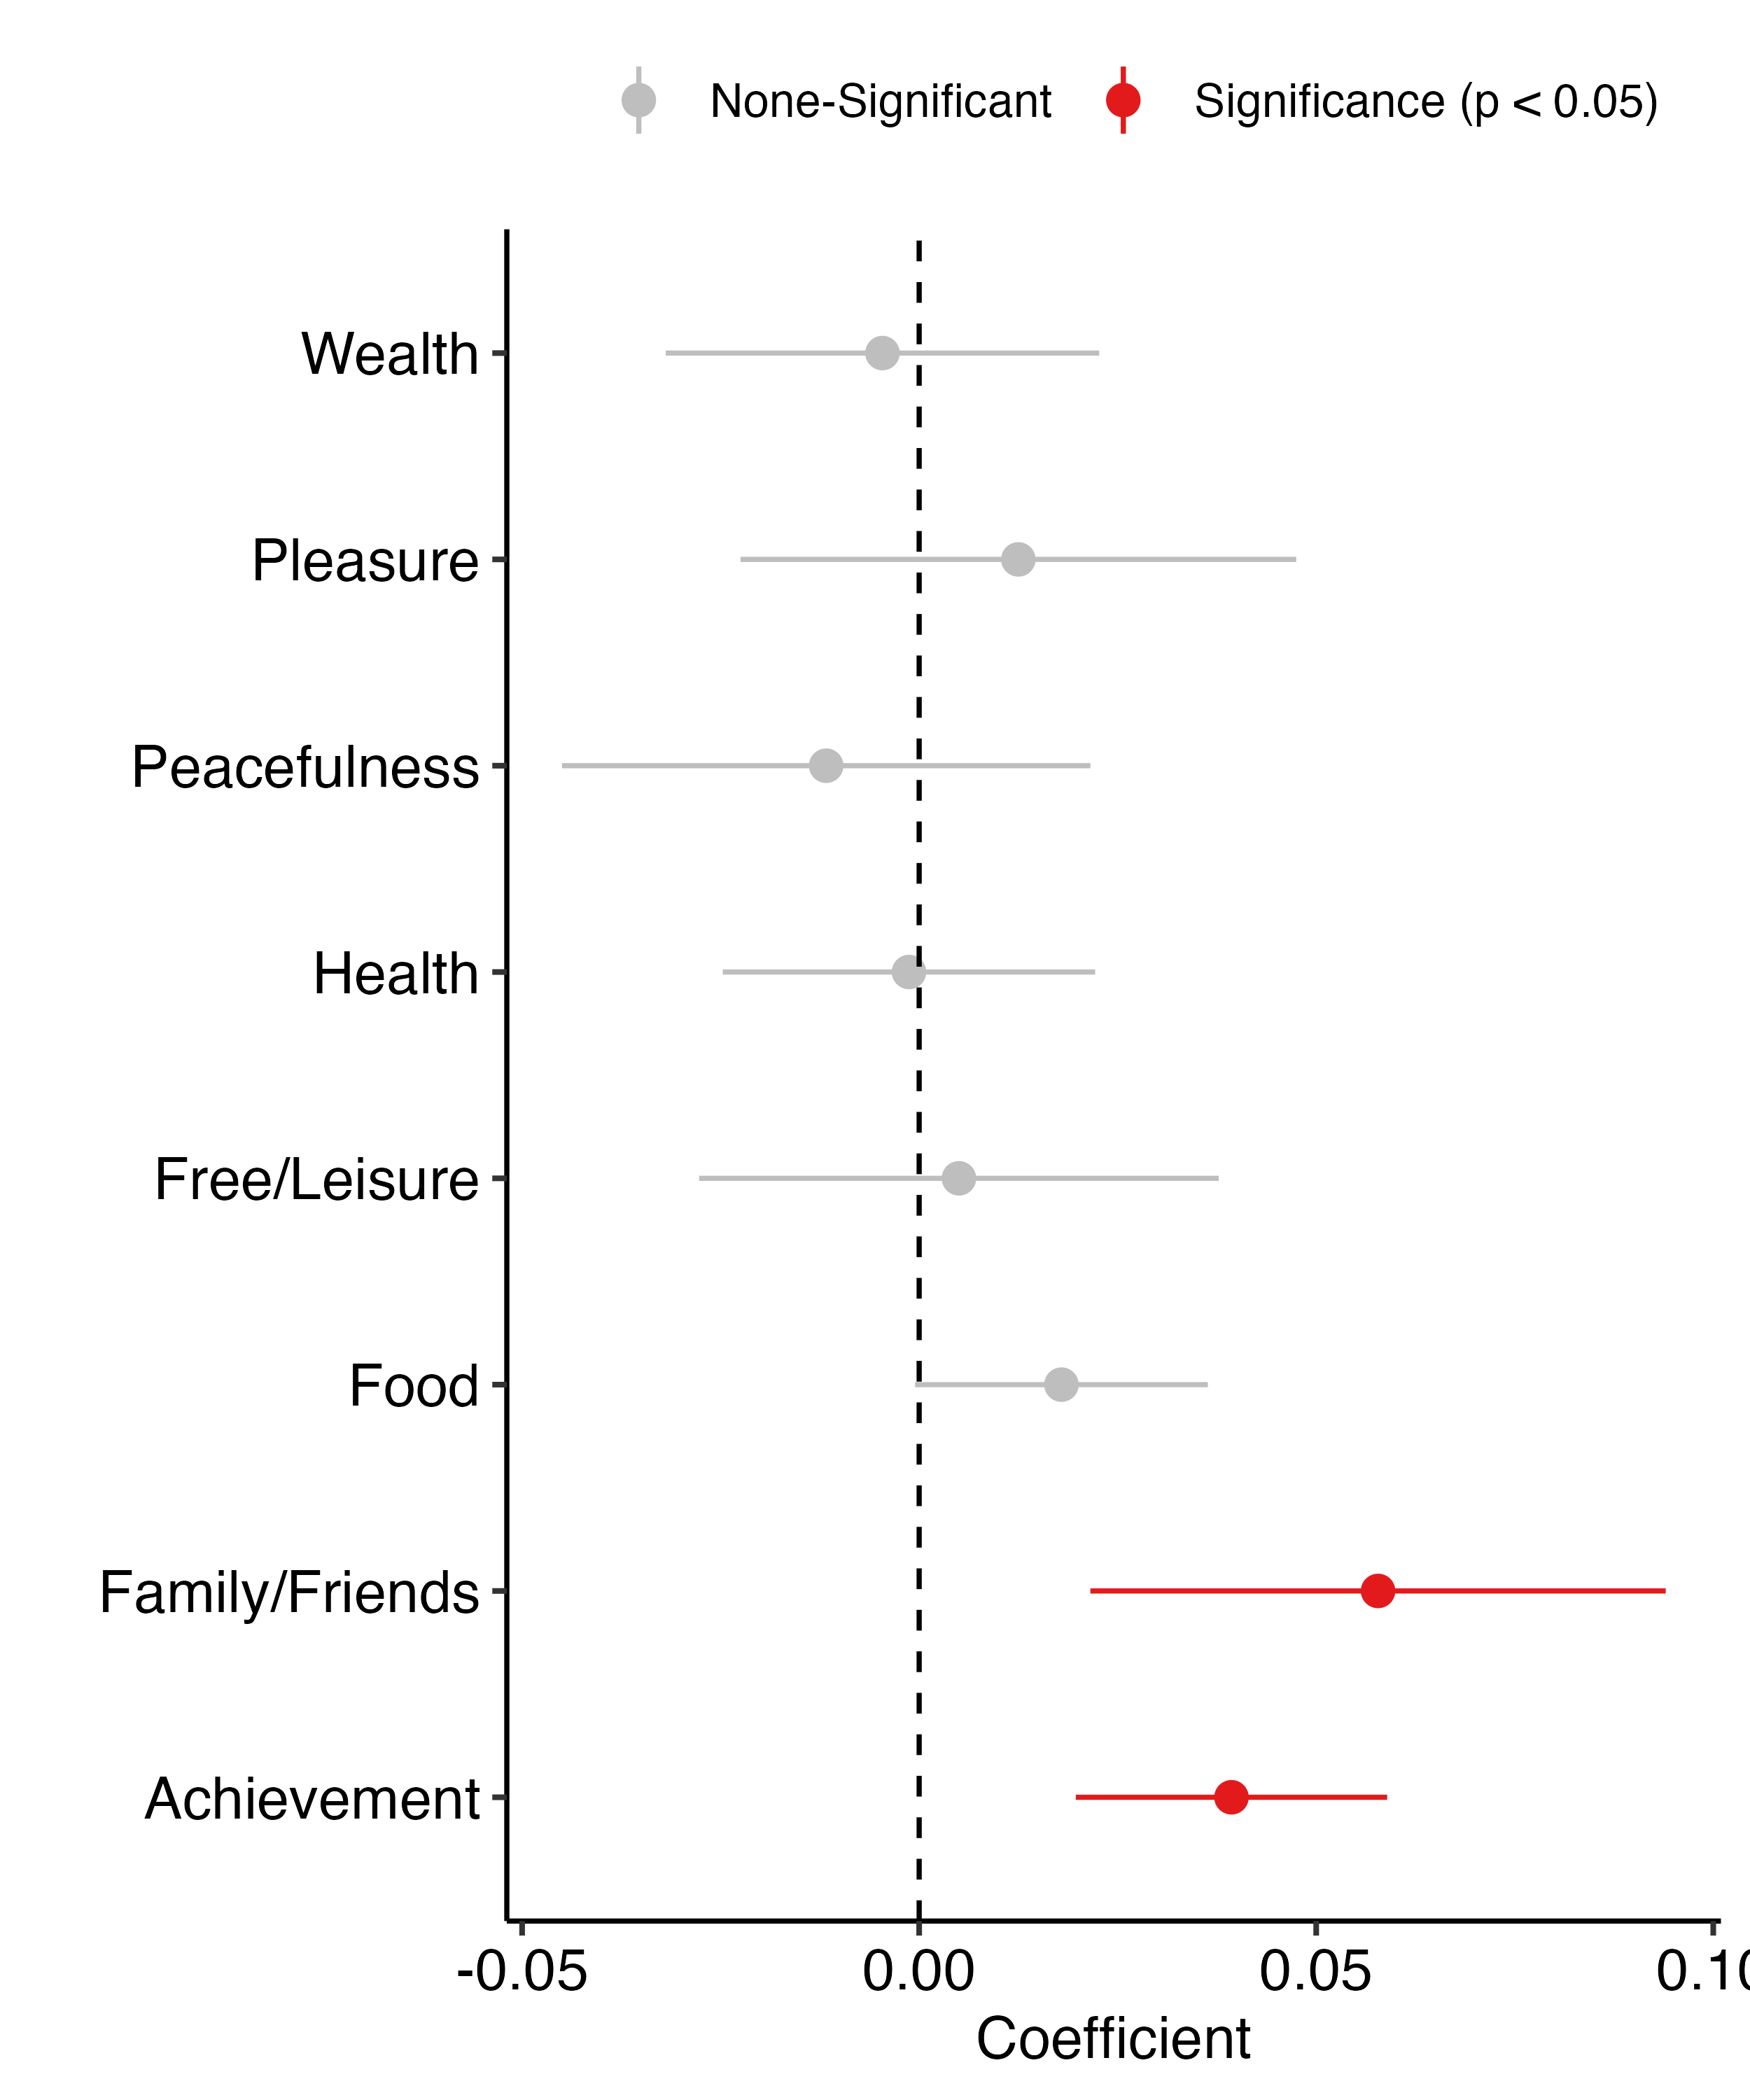
\includegraphics[width=\linewidth]{Images/well_being_community_income.png} % Trimming is used to crop your image and the order of dimensions is: left, bottom, right, top. It's recommended to crop outside of LaTeX though, to ensure the aspect ratio remains the same.
			%{\tiny\textcolor{ICLBlue}{(Above) Photography Credit or Caption}}
		\end{column}
	\end{columns}
\end{frame}

%------------------------------------------------

%------------------------------------------------
\subsection{Demographic differences in the perception of well-being from semantic perspectives}

%------------------------------------------------
%------------------------------------------------
\begin{frame}
    \frametitle{Analysis on demographic differences}
    \framesubtitle{Demographic differences from semantic perspectives}
    \begin{itemize}
        \item \textbf{Motivation}: Even within the context of identical components, the emphasis placed on specific aspects varies among different demographic groups, and this nuance is typically reflected in the \structure{semantic meanings of proposed words.}
        
        \item Estimate the effect of demographic characteristics on proposed words
    \end{itemize}
    
    $$
        logit(O_{ij}) = \beta_{0}+\beta_{1}X_{j}+\epsilon
    $$
    
    \vspace{-1.5\baselineskip}
    \begin{itemize}
        \item \structure{$O_{ij}$ implies the occurrence of word $i$ in the words proposed by participant $j$}
        \item $X_{j}$ refers to the demographic characteristics of participant $j$
        \begin{itemize}
            \item Gender: $1$ indicates male and $0$ indicates female.
            \item Age: Categorized into ranges from the 20s to the 70s, with the 20s serving as the reference category in the model. 
            \item Education attainment: Categorical variable converted into the numerical format, representing levels from \textit{junior high school} ($1$) to \textit{graduate school} ($6$)
            \item Income: Categorical variable converted into the numerical format, indicating income levels from \textit{no income} ($1$) to \textit{over 12 million yen per year} ($15$).
        \end{itemize}
    \end{itemize}
    
\end{frame}
%------------------------------------------------
%------------------------------------------------
\begin{frame}
	\frametitle{Analysis on demographic differences}
	\framesubtitle{Semantic difference in the perception of Family/Friends between males and females}
	\begin{columns}[T] % [T] ensures correct vertical alignment
		\begin{column}{0.48\linewidth} % Right column
			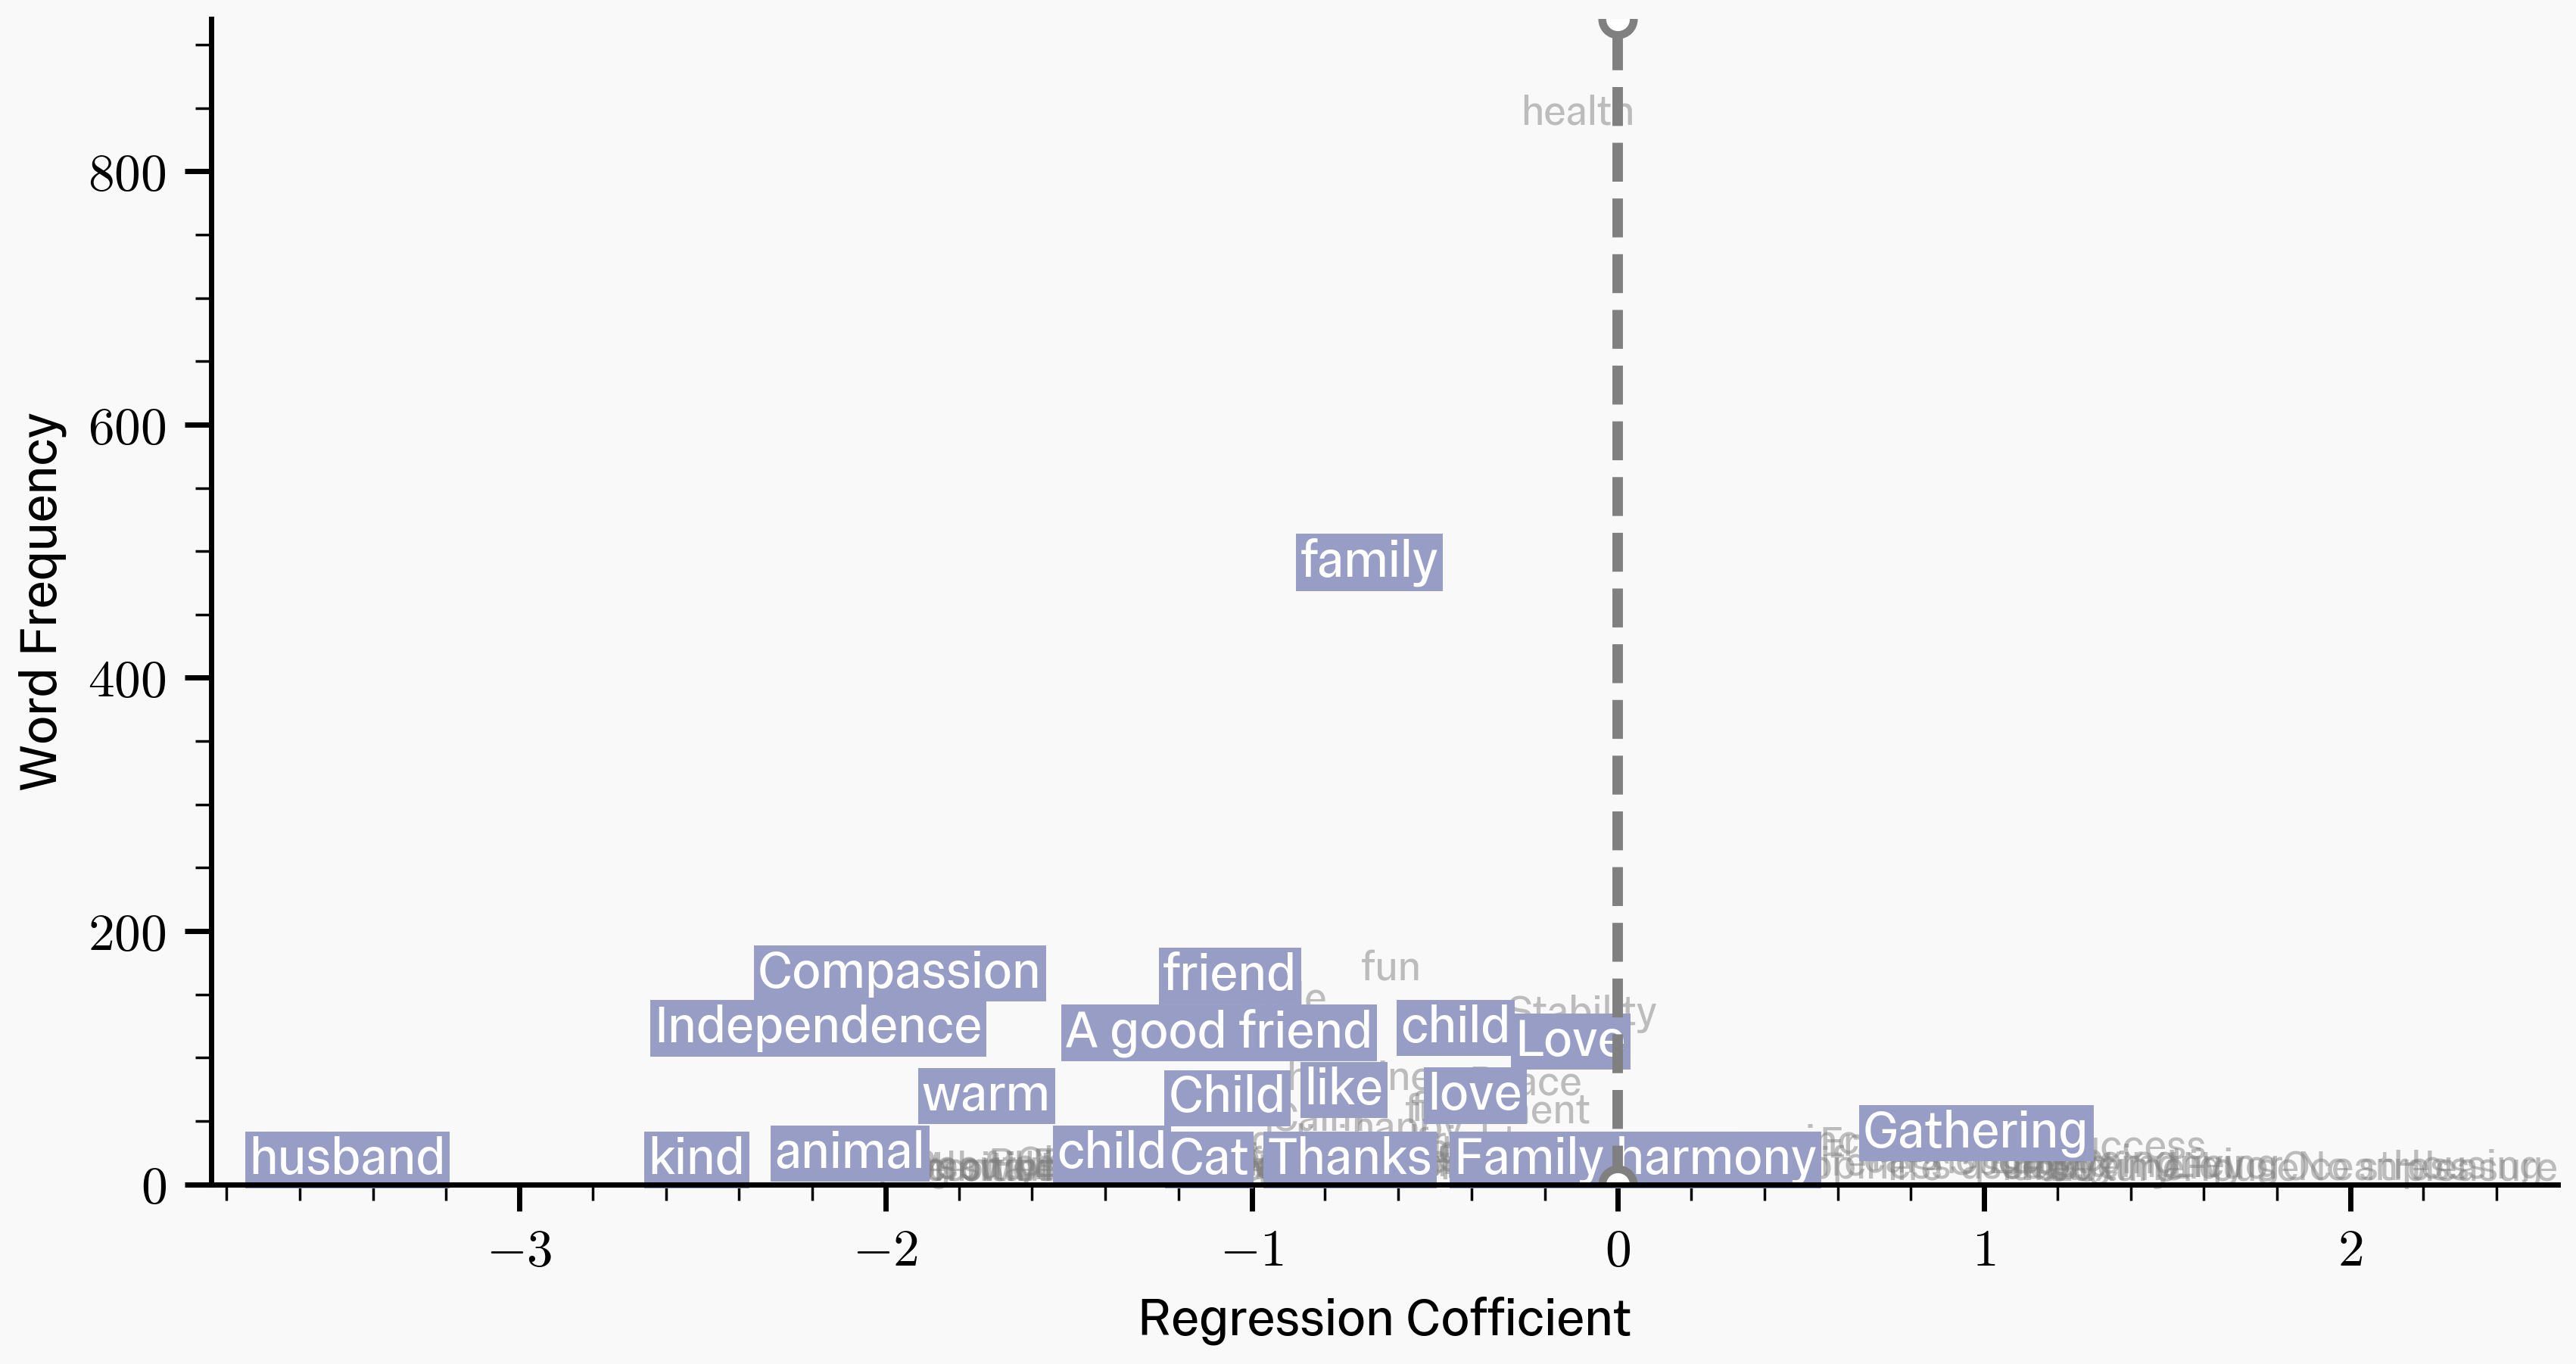
\includegraphics[width=\linewidth]{Images/gender_family_en.png} 
            \vspace{-1.5\baselineskip} 
            \begin{itemize}
                \item Words with statistically significant coefficients in the text regression are highlighted.
                \begin{itemize}
                    \item The original answer is in Japanese, translated by Google Translation 
                \end{itemize}

            \end{itemize}
		\end{column}
            \pause
            \begin{column}{0.48\linewidth} % Left column
			%\textbf{Inter-community connections}
                \vspace{1\baselineskip}
                Females tend to place a greater emphasis on interpersonal connections than males, while it is unclear who exactly is included in these supportive connections.
                \pause
                \begin{itemize}
                    \item  “\textit{family}” , “\textit{friends}” and “\textit{love}”  are more likely to be proposed by females.
                    \item  “\textit{animals}” and “\textit{cat}”
                    \begin{itemize}
                        \item Animals are increasingly being recognized as a source of emotional support and considered by many owners as friends and affectionate family members \citep{meehan_using_2017}.                        
                    \end{itemize}
 
                \end{itemize}
		\end{column}
	\end{columns}
\end{frame}
%------------------------------------------------

%------------------------------------------------
\begin{frame}
	\frametitle{Analysis on demographic differences}
	\framesubtitle{Semantic difference in the perception of Wealth between males and females}
	\begin{columns}[T] % [T] ensures correct vertical alignment
		\begin{column}{0.48\linewidth} % Right column
			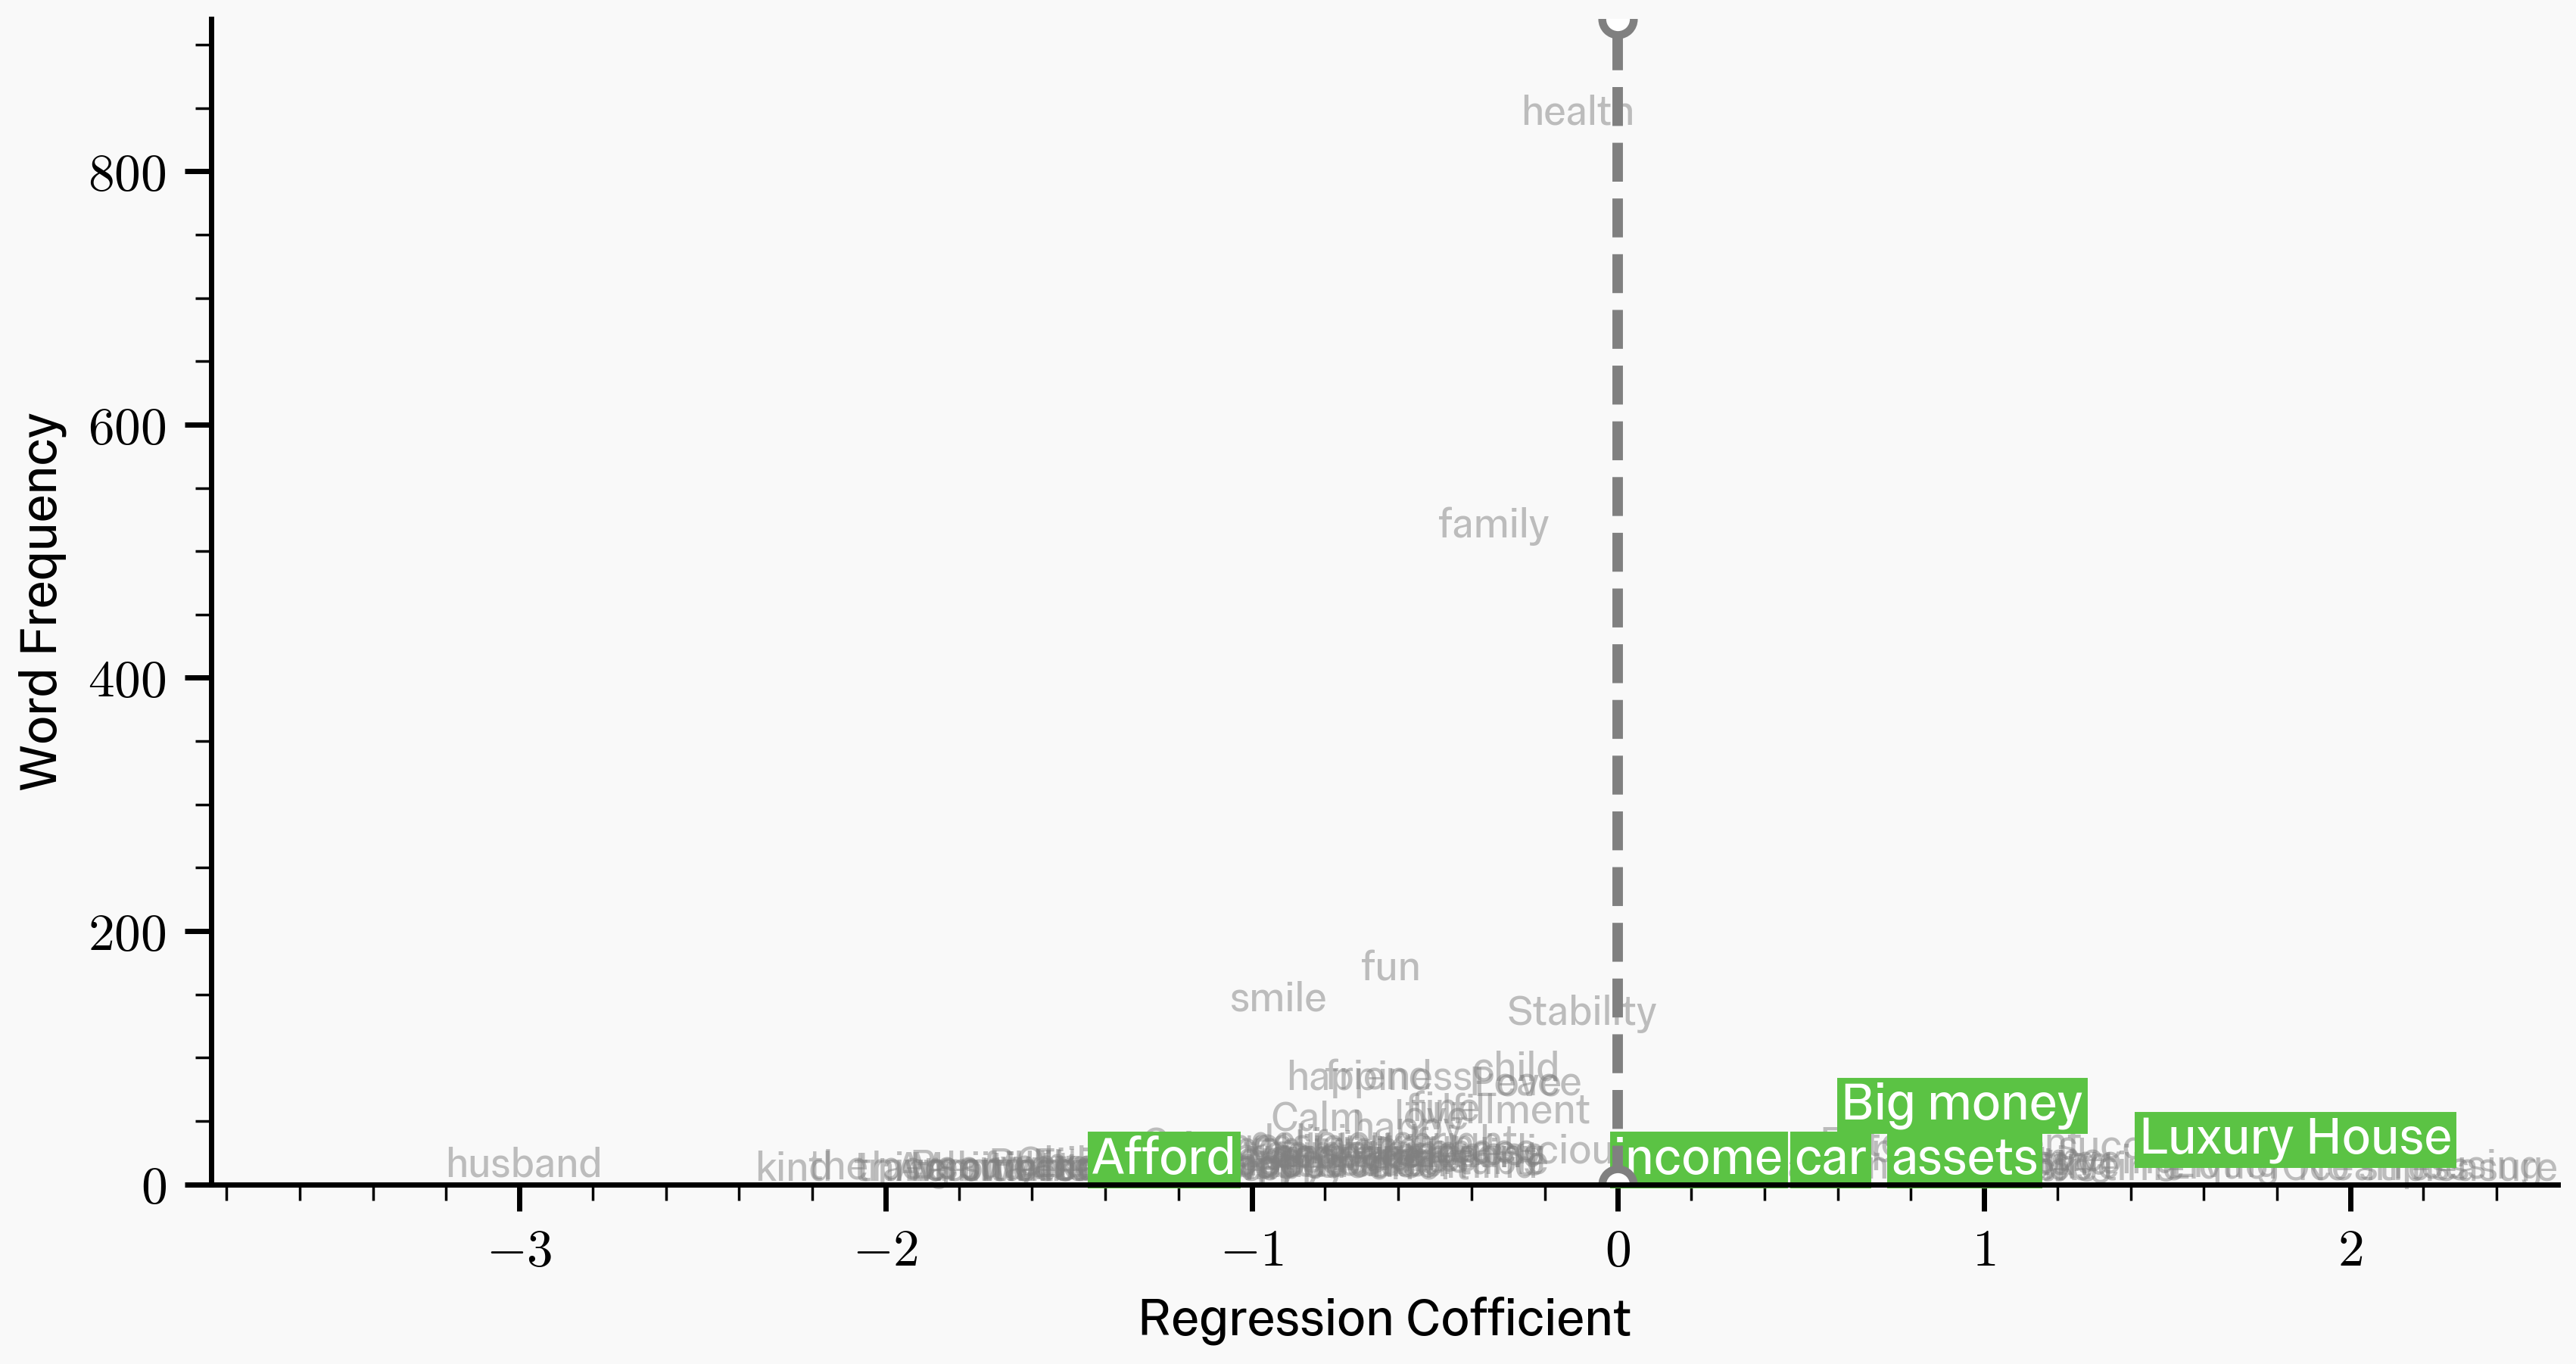
\includegraphics[width=\linewidth]{Images/plot_regression_wealth_en.png} 
            \vspace{-1.5\baselineskip} 
            \begin{itemize}
                \item Words with statistically significant coefficients in the text regression are highlighted.
                \begin{itemize}
                    \item The original answer is in Japanese, translated by Google Translation 
                \end{itemize}

            \end{itemize}
		\end{column}
            \begin{column}{0.48\linewidth} % Left column
			%\textbf{Inter-community connections}
                \vspace{1\baselineskip}
               Although previous analyses have indicated gender differences on a general level, further semantic analysis reveals more detailed underlying differences.
               \pause
                \begin{itemize}
                    \item  Males are more likely to place greater importance on \structure{material possessions that display their economic status}, such as "houses" and "cars". 
                    \item This tendency reflects societal expectations for males to demonstrate success and stability through visible symbols of wealth and achievement.
 
                \end{itemize}
		\end{column}
	\end{columns}
\end{frame}
%------------------------------------------------
\section{Discussion}
%------------------------------------------------
\begin{frame}
	\frametitle{Discussion}
        \framesubtitle{Implications}
        \begin{itemize}
            \item \textbf{Offer a analysis framework to more comprehensively understand well-being through exploratory analysis.}
            \begin{itemize}
                \item Measurement with pre-defined categories may be incomplete, especially since the components well-being may be context-dependent.
                \item Exploratory analysis can more efficiently deconstruct complex concepts and uncover aspects that may be overlooked
            \end{itemize}
            \pause
            \item \textbf{Enables a more detailed investigation of demographic differences.}
            \begin{itemize}
                \item The structure of word-association network provides a macroscopic view of how different components are interconnected across demographic groups.
                \item Semantic details offer a closer insights into the meanings and nuances of words within these connections.
            \end{itemize}
        \end{itemize}
\end{frame}

%------------------------------------------------

%------------------------------------------------
\begin{frame}
	\frametitle{Discussion}
        \framesubtitle{Future directions}
        \begin{itemize}
            \item The proposed method and analysis framework possess broad universality and applicability, and thus can be effectively leveraged in deconstructing and analyzing various complex concepts.
            \begin{itemize}
                \item Simplify the process for researchers by only requiring them to guide participants to complete word association tasks during data collection.
                \item Avoids the extensive efforts typically required to pre-define, delineate, and analyze complex concepts, streamlining the research process significantly
            \end{itemize}
            \item We have used the same method to investigate ill-being.
        \end{itemize}
\end{frame}


%----------------------------------------------------------------------------------------

\begin{frame}[allowframebreaks]{Bibliography}
\bibliography{references.bib}
\end{frame}

\begingroup
	\setbeamercolor{normal text}{fg=ICLBlue}\usebeamercolor[fg]{normal text} % Slide text color
	%\setbeamertemplate{closing slide logo}[logo]{ICL_Logo_Blue.pdf} % Imperial logo color, use 'ICL_Logo_White.pdf' for white and 'ICL_Logo_Blue.pdf' for blue
	\setbeamertemplate{closing slide text}[text]{Thanks for your attention!} % Slide text
	\usebeamertemplate{closing slide} % Output the closing slide
\endgroup

\end{document}
